%%ORIGEN: chapters/chapter03.tex, \chapter{Tecnologías} (líneas 467-675). Obsoleto, reemplazado por arquitectura.tex
\chapter{Tecnologías}
\label{sec:tecnologias}
Para cada tecnología se explica no solo cuál fue utilizada, sino también el motivo de su elección frente a otras alternativas posibles, considerando las necesidades y características concretas del proyecto.

El sistema calcula un \emph{score} de riesgo para cada usuario a partir de distintos eventos de comportamiento, mantiene el estado operativo en tiempo real, guarda un historial diario de los datos procesados y permite consultar la información mediante un \emph{dashboard}. Además, cuenta con un agente local encargado de aplicar las medidas de mitigación definidas por el sistema, cumpliendo el rol de \emph{Policy Enforcement Point} (PEP).

Debido a esta distribución de responsabilidades, el proyecto no está planteado como una aplicación monolítica, sino como un sistema compuesto por varios componentes que trabajan de manera conjunta; por eso las tecnologías utilizadas en cada parte fueron seleccionadas teniendo en cuenta la función que cumple cada componente dentro de la arquitectura general. El proyecto está organizado como un \emph{monorepo} que contiene cinco subsistemas principales: la API encargada del \emph{scoring} en tiempo real (\texttt{api/}), el agente PEP local (\texttt{agent/}), el \emph{dashboard} web (\texttt{frontend/}), el \emph{pipeline} de entrenamiento offline del modelo (\texttt{ml\_core/}), los \emph{scripts} de demostraciones, reproducción de eventos y validaciones (\texttt{scripts/}).

\section{Lenguajes de programación}
La elección de lenguajes del proyecto no es uniforme: cada componente utiliza el lenguaje que mejor se ajusta a su función y a su entorno de ejecución.

\begin{longtable}{p{2.4cm}p{4.4cm}p{7.8cm}}
	\caption{Lenguajes de programación utilizados}
	\label{tab:lenguajes}\\
	\hline
	\textbf{Lenguaje} & \textbf{Dónde se usa} & \textbf{Justificación} \\
	\hline
	\endfirsthead
	\hline
	\textbf{Lenguaje} & \textbf{Dónde se usa} & \textbf{Justificación} \\
	\hline
	\endhead
	Python 3.11 & API de \emph{scoring} (\texttt{api/}), agente (\texttt{agent/}), \emph{pipeline} offline (\texttt{ml\_core/}, \texttt{scripts/}) & Es el lenguaje utilizado en todo el \emph{pipeline} de procesamiento de datos y desarrollo de los modelos de \emph{machine learning}, incluyendo los \emph{notebooks} de las distintas fases, \texttt{scikit-learn} y TensorFlow. Mantener Python tanto en el entrenamiento como en la API de producción permite reutilizar directamente código ya desarrollado y validado en etapas anteriores (por ejemplo, \texttt{api/app/scoring/artifacts.py} incorpora \texttt{scripts/} al \texttt{sys.path} para importar \texttt{\_score\_common.py} y \texttt{\_audit\_common.py}), evitando reimplementar en otro lenguaje la lógica matemática del \emph{score} híbrido y reduciendo el riesgo de diferencias entre lo validado en entrenamiento y lo ejecutado en producción. \\
	\hline
	TypeScript & \emph{Dashboard} (\texttt{frontend/}) & El \emph{frontend} maneja estructuras de datos relativamente complejas (\texttt{EventoScoreOut}, \texttt{UmbralesConfig}, \texttt{AccionesConfig}, \texttt{ReentrenamientoConfig}) y permite modificar configuraciones que afectan directamente el comportamiento del agente, como los umbrales de riesgo y la relación entre cada nivel y la acción a ejecutar. Un error en la estructura de los datos podría generar problemas reales (por ejemplo, que el agente reciba un \texttt{accion\_id} incorrecto), por lo que se usa TypeScript para detectar problemas en tiempo de desarrollo, junto con Zod para validar los datos recibidos en tiempo de ejecución mediante \texttt{schema.parse()}. Esta doble capa de control aporta mayor seguridad y confiabilidad que trabajar únicamente con JavaScript. \\
	\hline
	PowerShell & \url{scripts/install_agent_task.ps1} y \url{uninstall_agent_task.ps1} & Es el lenguaje nativo de automatización de Windows (\texttt{schtasks}). El agente PEP es exclusivamente Windows por diseño (necesita \texttt{icacls} para ACLs de carpeta y \texttt{psutil}/la API de Windows para terminar procesos), por lo que registrar su arranque automático mediante la herramienta nativa del propio sistema operativo es la opción consistente, en vez de introducir un tercer lenguaje de automatización genérico. \\
	\hline
\end{longtable}

\noindent\textbf{Alternativas consideradas y descartadas:}
\begin{itemize}
	\item \emph{Backend} en Node.js/TypeScript: se consideró usar un único lenguaje para todo el sistema, pero se descartó. Si bien Node.js/TypeScript es una buena opción para el desarrollo de APIs, Python ofrece soluciones mucho más completas para \emph{machine learning}, en especial para trabajar con modelos como Isolation Forest y \emph{autoencoders} LSTM; usar Node.js para todo el \emph{backend} habría requerido igualmente un servicio separado en Python para la parte de \emph{machine learning}.
	\item Java / Spring Boot para la API: también se evaluó, pero se decidió no hacerlo, ya que para el alcance de este proyecto implicaba una mayor cantidad de configuración y código adicional.
\end{itemize}

\section{Frameworks y librerías}
Se detallan a continuación los \emph{frameworks} y librerías utilizados en cada subsistema, agrupados según su función dentro del proyecto: la API de \emph{scoring}, el agente PEP, el \emph{frontend} y el \emph{pipeline} de entrenamiento offline.

\subsection{API de Scoring (api/)}
\begin{longtable}{p{3cm}p{11.6cm}}
	\caption{Frameworks y librerías: API de \emph{Scoring}}
	\label{tab:frameworks-api}\\
	\hline
	\textbf{Tecnología} & \textbf{Justificación} \\
	\hline
	\endfirsthead
	\hline
	\textbf{Tecnología} & \textbf{Justificación} \\
	\hline
	\endhead
	FastAPI & Soporte \emph{async} nativo, necesario porque cada evento dispara E/S hacia Redis y, al cerrar el día, hacia Postgres, sin bloquear el resto de las \emph{requests} concurrentes. Ofrece además validación automática de entrada/salida vía Pydantic y generación gratuita de documentación OpenAPI, útil para una API con 11 \emph{endpoints} documentados formalmente. Frente a Flask: Flask no tiene \emph{async} nativo ni validación de esquemas integrada; habría que sumar extensiones para llegar al mismo punto. \\
	\hline
	Uvicorn & Servidor utilizado para ejecutar la API desarrollada con FastAPI. Se eligió porque está diseñado para trabajar directamente con FastAPI y permite gestionar las solicitudes y respuestas de la API de forma eficiente. \\
	\hline
	Pydantic v2 & Define los contratos de datos (\texttt{EventoIn}, \texttt{EventoScoreOut}, \texttt{UmbralesConfig}, \texttt{AccionesConfig}, \texttt{ReentrenamientoConfig}) que cruzan el límite entre agente, API y \emph{dashboard}. Un \emph{payload} mal formado se rechaza automáticamente con código 422, sin necesidad de código de validación manual. \\
	\hline
	SQLAlchemy + psycopg2-binary & Acceso a Postgres/Supabase para el historial de días cerrados (\texttt{historial\_scores}). SQLAlchemy abstrae el dialecto SQL concreto, permitiendo tratar Supabase como un Postgres estándar sin código específico del proveedor. El \emph{pool} de conexiones está ajustado a un volumen bajo de escrituras coherente con que la escritura solo ocurre al cerrar un día calendario, no por cada evento. \\
	\hline
	redis-py & Cliente de Redis para el estado en caliente por usuario. Se eligió Redis sobre Postgres porque el \emph{hot path} (una escritura de estado por cada evento recibido, potencialmente cientos por usuario y por día) es un patrón de lectura/escritura de baja latencia y alta frecuencia, distinto del historial agregado (una escritura por usuario y por día). Concentrar ambos patrones en la misma base relacional habría sobrecargado una base pensada para consultas transaccionales, no para actualizaciones de estado de alta frecuencia. Redis permite además concurrencia optimista nativa (\texttt{WATCH}/\texttt{MULTI}/\texttt{EXEC}), que \texttt{redis\_state.py} utiliza para reintentar hasta 5 veces ante colisiones de escritura concurrente. \\
	\hline
	scikit-learn (IsolationForest) & Implementación madura y bien documentada de detección de anomalías no supervisada sobre el agregado diario de actividad. Se eligió sobre alternativas más recientes (\emph{autoencoders} tabulares, \emph{one-class SVM}) porque es computacionalmente liviano, no requiere ajustar una arquitectura de red neuronal para datos tabulares agregados, y da una salida interpretable (\texttt{decision\_function}) que luego se usa para la explicabilidad del \emph{score}. \\
	\hline
	TensorFlow / Keras (LSTM Autoencoder) & Necesario porque Isolation Forest trabaja sobre datos agregados y no tiene en cuenta el orden en que ocurren los eventos dentro de una sesión. El LSTM Autoencoder permite analizar secuencias de eventos consecutivos, por lo que puede detectar comportamientos anómalos que podrían pasar desapercibidos al analizar únicamente el total de actividad de un día. Por ejemplo, una secuencia inusual de acciones puede ser anómala aunque el volumen total de actividad del usuario sea normal.

Frente a PyTorch: se eligió Keras por ofrecer una API de alto nivel que simplifica la implementación y el entrenamiento del LSTM Autoencoder, reduciendo la complejidad del desarrollo y mantenimiento del modelo. \\
	\hline
	pandas, numpy, scipy, joblib & Manipulación tabular y numérica en los \emph{notebooks} de las fases 1 a 6; \texttt{joblib} se usa específicamente para serializar/deserializar el IsolationForest entrenado (\texttt{isolation\_forest.joblib}) de forma eficiente. \\
	\hline
\end{longtable}

\subsection{Agente (agent/)}
\begin{longtable}{p{3cm}p{11.6cm}}
	\caption{Frameworks y librerías: Agente}
	\label{tab:frameworks-agente}\\
	\hline
	\textbf{Tecnología} & \textbf{Justificación} \\
	\hline
	\endfirsthead
	\hline
	\textbf{Tecnología} & \textbf{Justificación} \\
	\hline
	\endhead
	requests & Cliente HTTP utilizado por ScoringClient para enviar eventos a la API mediante solicitudes POST. Se eligió por su simplicidad y porque el agente realiza las solicitudes de forma secuencial, sin necesidad de manejar múltiples solicitudes simultáneamente. \\
	\hline
	psutil & Única forma multiplataforma madura de enumerar procesos y conexiones de red desde Python sin llamar directo a la API de Windows. Es deliberadamente la única dependencia no-\emph{stdlib} además de \texttt{requests} (\texttt{agent/requirements.txt} tiene solo dos líneas): el agente corre en el \emph{endpoint} del usuario final, así que minimizar dependencias reduce la superficie de ataque y el \emph{footprint} del proceso que se ejecuta en segundo plano todo el día. \\
	\hline
\end{longtable}

\subsection{Frontend (frontend/)}
\begin{longtable}{p{3cm}p{11.6cm}}
	\caption{Frameworks y librerías: \emph{Frontend}}
	\label{tab:frameworks-frontend}\\
	\hline
	\textbf{Tecnología} & \textbf{Justificación} \\
	\hline
	\endfirsthead
	\hline
	\textbf{Tecnología} & \textbf{Justificación} \\
	\hline
	\endhead
	React 19 & Modelo de componentes reutilizables adecuado para un \emph{dashboard} con piezas repetidas entre vistas (\texttt{RiskBadge}, \texttt{CoverageBadge}, \texttt{LoadingState}, \texttt{ErrorState} se reutilizan en las cinco páginas del sistema). \\
	\hline
	Vite & Tiempos de arranque y \emph{hot module reload} sensiblemente más rápidos que Create React App/Webpack para un proyecto de este tamaño, algo relevante en el ciclo de desarrollo acotado de una tesis. \\
	\hline
	TypeScript + zod & Ver justificación detallada en la sección de Lenguajes: doble validación entre compilación y \emph{runtime}. \\
	\hline
	TanStack Query v5 & Maneja \emph{cacheo}, revalidación y \emph{polling} (cada 7 segundos) de los datos remotos sin escribir a mano la lógica de \emph{refetch}, estado de carga y error para cada una de las 7 consultas del \emph{dashboard}. Es también lo que permite el patrón \texttt{useMutation} con \texttt{setQueryData} para reflejar al instante en la interfaz un cambio de umbrales recién guardado, sin esperar al próximo ciclo de \emph{polling}. \\
	\hline
	React Router v7 & Enrutamiento estándar de \emph{SPA} para las 5 vistas del \emph{dashboard}: listado de usuarios, detalle de usuario, historial, umbrales y salud del sistema. \\
	\hline
	Recharts & Gráfico de evolución de riesgo (\texttt{RiskTimeline}): librería declarativa que se integra de forma natural con el modelo de componentes de React, evitando manipular un \emph{canvas} o SVG a mano para un gráfico de líneas simple. \\
	\hline
	Tailwind CSS 4 & Sistema de utilidades para implementar el tema claro/oscuro (\texttt{data-theme}) mediante \emph{custom properties}, sin mantener hojas de estilo separadas por tema. \\
	\hline
	Oxlint & \emph{Linter} utilizado para detectar errores y mantener buenas prácticas en el código del frontend. Se eligió principalmente por su rapidez y facilidad de integración, siendo una alternativa adecuada para un proyecto con tiempo de desarrollo limitado.\\
	\hline
\end{longtable}

\subsection{Pipeline offline (ml\_core/, scripts/)}
\begin{longtable}{p{3cm}p{11.6cm}}
	\caption{Frameworks y librerías: \emph{Pipeline} offline}
	\label{tab:frameworks-mlcore}\\
	\hline
	\textbf{Tecnología} & \textbf{Justificación} \\
	\hline
	\endfirsthead
	\hline
	\textbf{Tecnología} & \textbf{Justificación} \\
	\hline
	\endhead
	DuckDB & Motor analítico embebido que ejecuta consultas tipo SQL sobre \texttt{data/clue.json} (14~GB, \emph{JSON Lines}) sin cargarlo entero en memoria ni levantar un motor de base de datos separado solo para extraer historiales puntuales de usuario. Es la herramienta correcta para ``una consulta puntual sobre un archivo grande'', frente a montar Postgres o Spark para ese mismo propósito. \\
	\hline
	imbalanced-learn & Declarada en \texttt{ml\_core/requirements.txt}, es coherente con que el \emph{dataset} de entrenamiento tiene una proporción de eventos anómalos extremadamente baja (253 sesiones etiquetadas sobre 7,6 millones de eventos), un escenario típico donde se necesitan técnicas de balanceo de clases. \\
	\hline
	Jupyter / ipykernel & Los \emph{notebooks} Fase 1 a Fase 6 constituyen el \emph{pipeline} real de preparación de datos y entrenamiento. La elección de \emph{notebooks} por sobre \emph{scripts} puros para esta parte responde a que es trabajo exploratorio e iterativo: no hay ejecución \emph{headless} documentada, es un flujo manual e interactivo por diseño en esta etapa del proyecto, no en producción. \\
	\hline
\end{longtable}

\section{Arquitectura de red}

\subsection{Topología general}
El sistema no está diseñado como una aplicación monolítica que se ejecuta en un único entorno, sino compuesto por varios componentes, cada uno con una función específica y con distintas necesidades de despliegue. La API, Redis, el \emph{frontend} y el \emph{pipeline} de entrenamiento (\texttt{ml\_core}) se ejecutan mediante Docker Compose, lo que permite mantener estos servicios organizados dentro de una misma red virtual y facilita su puesta en funcionamiento. Por otro lado, la base de datos utilizada para almacenar el historial se encuentra fuera de esta infraestructura y se utiliza como un servicio gestionado de PostgreSQL mediante Supabase. El agente PEP (\texttt{agent/}) tiene un tratamiento diferente: se ejecuta directamente en el equipo Windows del usuario final y permanece fuera de los contenedores, ya que necesita acceder a recursos del sistema operativo, como procesos y permisos sobre archivos.

\begin{verbatim}
+------------------------- Docker Compose -------------------------+
|                                                                   |
|   +----------+      +--------------+      +-----------+          |
|   | frontend |<---->|     api      |<---->|   redis   |          |
|   | (Vite)   | CORS |  (FastAPI)   |      |           |          |
|   +----------+      +------+-------+      +-----------+          |
|                             |                                    |
|                      +------+-------+                            |
|                      |   ml_core    |  (entrenamiento offline)   |
|                      +--------------+                            |
+----------------------------+--------------------------------------+
                              | HTTP saliente (WAN)
                              v
                   +---------------------+
                   | Postgres / Supabase |  (servicio gestionado externo)
                   +---------------------+
                              ^
                              | HTTP (POST /eventos)
                   +----------+----------+
                   |   agent/ (host)     |  <- FUERA de Docker, por diseño
                   |   Windows endpoint  |
                   +---------------------+
\end{verbatim}

Dentro de Docker Compose, el \emph{frontend} se comunica con la API mediante HTTP, con CORS configurado para permitir las solicitudes desde el origen correspondiente. La API, a su vez, se comunica con Redis para mantener información de estado y con los componentes relacionados con el procesamiento y entrenamiento del modelo. La API también se comunica con PostgreSQL/Supabase, que funciona como almacenamiento persistente del historial; esta comunicación se realiza mediante la red externa, ya que se trata de un servicio gestionado que no forma parte de la infraestructura local del proyecto. Por último, el agente PEP se comunica con la API mediante HTTP, enviando principalmente los eventos generados en el \emph{endpoint}. Al ejecutarse directamente sobre Windows, el agente puede recibir las decisiones correspondientes y aplicar las medidas de mitigación sobre el equipo donde está instalado.

\subsection{Justificación de cada decisión de red}
\begin{itemize}
	\item \textbf{API + Redis + Frontend + ml\_core en Docker Compose, sobre un mismo host/red virtual:} estos componentes no dependen directamente del sistema operativo del usuario final, por lo que se decidió ejecutarlos mediante contenedores. Esto permite mantener un entorno reproducible, con las mismas versiones de las librerías y dependencias en las distintas máquinas donde se ejecute el proyecto. Además, Docker Compose facilita el inicio coordinado de los servicios mediante un único comando.
	\item \textbf{El agente queda deliberadamente fuera de Docker, corriendo nativo en el host Windows:} a diferencia del resto de los componentes, el agente se ejecuta de forma nativa en el sistema operativo del usuario. Esta decisión es especialmente importante porque el agente cumple el rol de \emph{Policy Enforcement Point} (PEP) y necesita interactuar directamente con recursos reales del \emph{endpoint} (entre otras tareas, puede finalizar procesos y modificar permisos mediante \texttt{icacls}). Si el agente estuviera dentro de un contenedor, quedaría aislado del sistema de archivos y de los procesos del host, lo que limitaría justamente las capacidades que necesita para funcionar como PEP; por este motivo, mantenerlo fuera de Docker no es una omisión, sino una decisión de diseño necesaria para este componente.
	\item \textbf{Postgres/Supabase como servicio externo gestionado, fuera del \texttt{docker-compose.yml} del proyecto:} de esta manera, la persistencia de los datos queda separada de la infraestructura utilizada para el desarrollo y las demostraciones. Esta decisión también es coherente con el enfoque del proyecto como un sistema distribuido y permite evitar la necesidad de administrar una instancia de base de datos local durante el desarrollo. La misma lógica se aplica a Redis mediante Upstash, utilizando servicios gestionados para reducir la infraestructura que debe mantenerse manualmente.
	\item \textbf{CORS explícito (\texttt{SCORING\_CORS\_ORIGINS}, por defecto \texttt{http://localhost:5173}):} durante el desarrollo, el \emph{frontend} se ejecuta en el puerto 5173, mientras que la API utiliza el puerto 8001. Al tratarse de dos orígenes diferentes, es necesario configurar CORS para permitir la comunicación entre ambos, lo que además permite que ambos componentes puedan desplegarse o modificarse de manera independiente.
	\item \textbf{Tres consumidores de red distintos hacia un mismo PDP central (agente, \emph{frontend}, \emph{scripts}), cada uno con su propio nivel de acceso:} el agente, el \emph{frontend} y los \emph{scripts} utilizan la API como punto central para acceder a las funcionalidades del sistema, aunque cada uno tiene permisos diferentes. El agente utiliza el nivel \emph{admin} para enviar eventos y realizar las operaciones que necesita para aplicar las políticas. El \emph{frontend} utiliza el nivel \emph{dashboard}, principalmente para consultar información y realizar algunas modificaciones de configuración específicas. Los \emph{scripts} pueden utilizar distintos modos según su objetivo: por ejemplo, \texttt{simulator.py} realiza comunicaciones HTTP reales, mientras que \texttt{run\_regression\_test.py} y \texttt{ensayo\_demo\_pep.py} pueden utilizar importaciones directas dentro del proceso para pruebas más rápidas, evitando el costo adicional de la comunicación por red.
\end{itemize}

\section{Protocolos de comunicación}
Cada enlace de comunicación entre componentes utiliza el protocolo o mecanismo más adecuado a la naturaleza de ese enlace: discreto o continuo, transaccional o de alta frecuencia, interno o hacia un servicio externo.

\begin{longtable}{p{3cm}p{3.5cm}p{8.1cm}}
	\caption{Protocolos de comunicación}
	\label{tab:protocolos}\\
	\hline
	\textbf{Protocolo / mecanismo} & \textbf{Dónde se usa} & \textbf{Justificación} \\
	\hline
	\endfirsthead
	\hline
	\textbf{Protocolo / mecanismo} & \textbf{Dónde se usa} & \textbf{Justificación} \\
	\hline
	\endhead
	HTTP/REST + JSON & Agente $\rightarrow$ API, \emph{Frontend} $\rightarrow$ API & Protocolo estándar, depurable con herramientas comunes (\texttt{curl}, Postman), con contratos de \emph{request}/\emph{response} bien definidos vía Pydantic en el \emph{backend} y \emph{zod} en el \emph{frontend}. El sistema trabaja con eventos discretos (un evento equivale a una \emph{request}), no con \emph{streams} continuos, por lo que REST sobre HTTP es el ajuste natural, sin necesidad de protocolos con estado persistente de conexión. \\
	\hline
	X-API-Key en dos \emph{tiers} (\emph{dashboard} / \emph{admin}) & Autenticación de todas las escrituras & La utilización de una \emph{API Key} no fue una decisión arbitraria. Durante el desarrollo se evaluó una alternativa basada en autenticación mediante \emph{login} y sesión/\emph{token}, que implicaba incorporar un \emph{endpoint} de autenticación y proteger los \emph{endpoints} de configuración. Esta alternativa llegó a implementarse y probarse, pero se decidió revertirla debido a problemas generados en el entorno de desarrollo (sin que existieran problemas con la lógica de funcionamiento); para el alcance actual del proyecto, orientado a una prueba de concepto, se priorizó una solución más simple y práctica mediante \emph{API Key}. Esta decisión es revisable: para una futura puesta en producción sería recomendable reemplazar este mecanismo por un sistema de autenticación más robusto, especialmente porque una \emph{API Key} incluida en el \emph{bundle} del \emph{frontend} puede quedar expuesta al usuario final. (Nota de alcance: mejora planteada para después del hito del 50\%, sujeta a los tiempos y alcance restante del proyecto.) \\
	\hline
	\emph{Polling} HTTP periódico (7~s) vía TanStack Query & \emph{Frontend} $\rightarrow$ API & El \emph{score} se recalcula por evento entrante y no existe un caso de uso que necesite empuje instantáneo al \emph{dashboard} (a diferencia, por ejemplo, de un chat). WebSockets habría agregado manejo de conexión persistente, reconexión y estado de \emph{socket} sin un beneficio proporcional al alcance de un \emph{dashboard} de administración que se refresca cada pocos segundos; se eligió esta opción por su simplicidad razonable para el alcance actual del proyecto. \\
	\hline
	RESP (\emph{Redis Serialization Protocol}) vía redis-py, con \texttt{WATCH}/\texttt{MULTI}/\texttt{EXEC} & API $\leftrightarrow$ Redis & Necesario para las actualizaciones atómicas y optimistas del estado por usuario bajo escritura concurrente (\texttt{update\_state()} reintenta hasta 5 veces ante colisión), evitando condiciones de carrera cuando llegan eventos del mismo usuario en rápida sucesión. \\
	\hline
	Protocolo \emph{wire} de PostgreSQL vía psycopg2 + SQLAlchemy & API $\rightarrow$ Postgres/Supabase & Estándar y maduro, con \emph{pool} de conexiones dimensionado al patrón de escritura real (una por día cerrado, no por evento). Los parámetros \texttt{connect\_timeout=3} y \texttt{pool\_pre\_ping=True} evitan que una caída de Postgres bloquee indefinidamente el \emph{hot path} de \emph{scoring}. \\
	\hline
	Ausencia declarada de TLS mutuo y de firma de respuestas del PDP & Agente $\leftrightarrow$ API & Actualmente, la falta de autenticación mutua entre el agente y el PDP se considera una limitación propia del alcance de esta etapa del proyecto y se encuentra documentada. Para una futura puesta en producción, sería recomendable resolver este punto mediante algún mecanismo de autenticación entre ambos componentes, de forma que puedan verificar su identidad antes de intercambiar información o recibir instrucciones. (Nota de alcance: mejora planteada para después del hito del 50\%, sujeta a los tiempos y alcance restante del proyecto.) \\
	\hline
\end{longtable}

\clearpage
%%ORIGEN: chapters/chapter03.tex, \chapter{Modelo de Datos} (líneas 676-705). Obsoleto, reemplazado por datos.tex
\chapter{Modelo de Datos}
\section{Diagrama de Bases de Datos}

\begin{figure}[h]
	\centering
	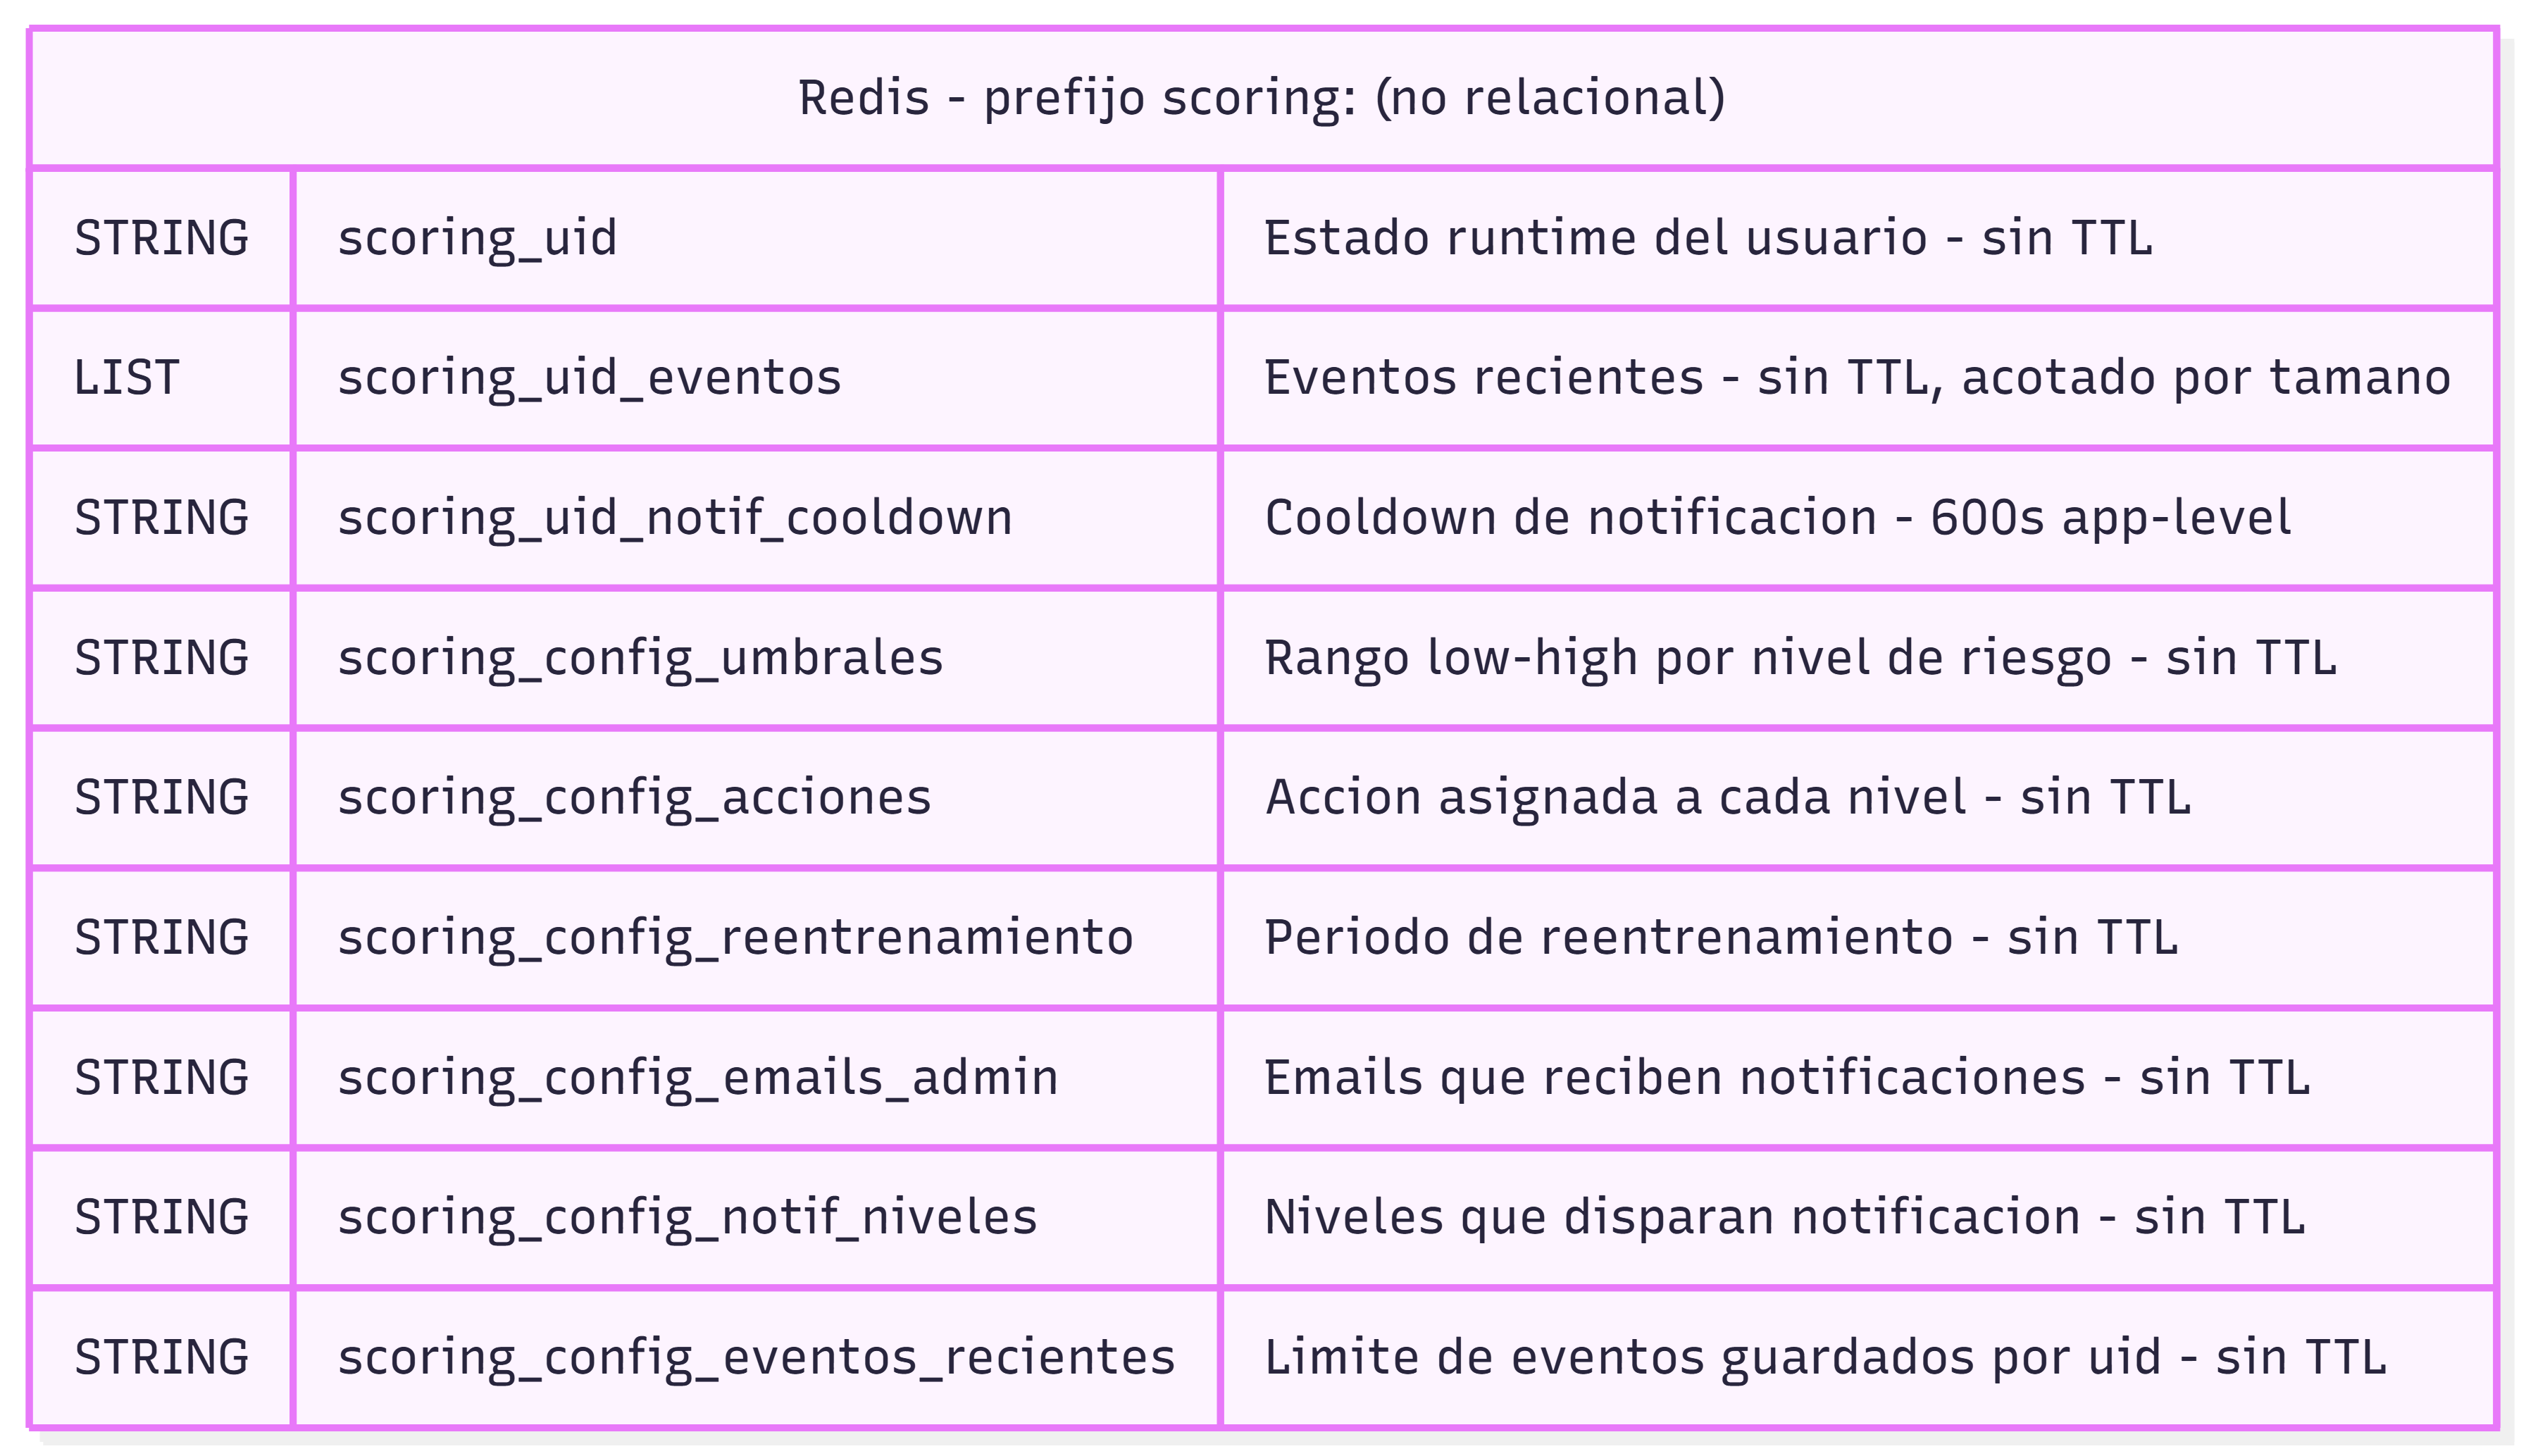
\includegraphics[width=\textwidth]{images/diagramas/redis.png}
	\caption{Diagrama de Bases de Datos.}
	\label{fig:diagrama-bases-de-datos-redis}
\end{figure}
\FloatBarrier

\begin{figure}[h]
	\centering
	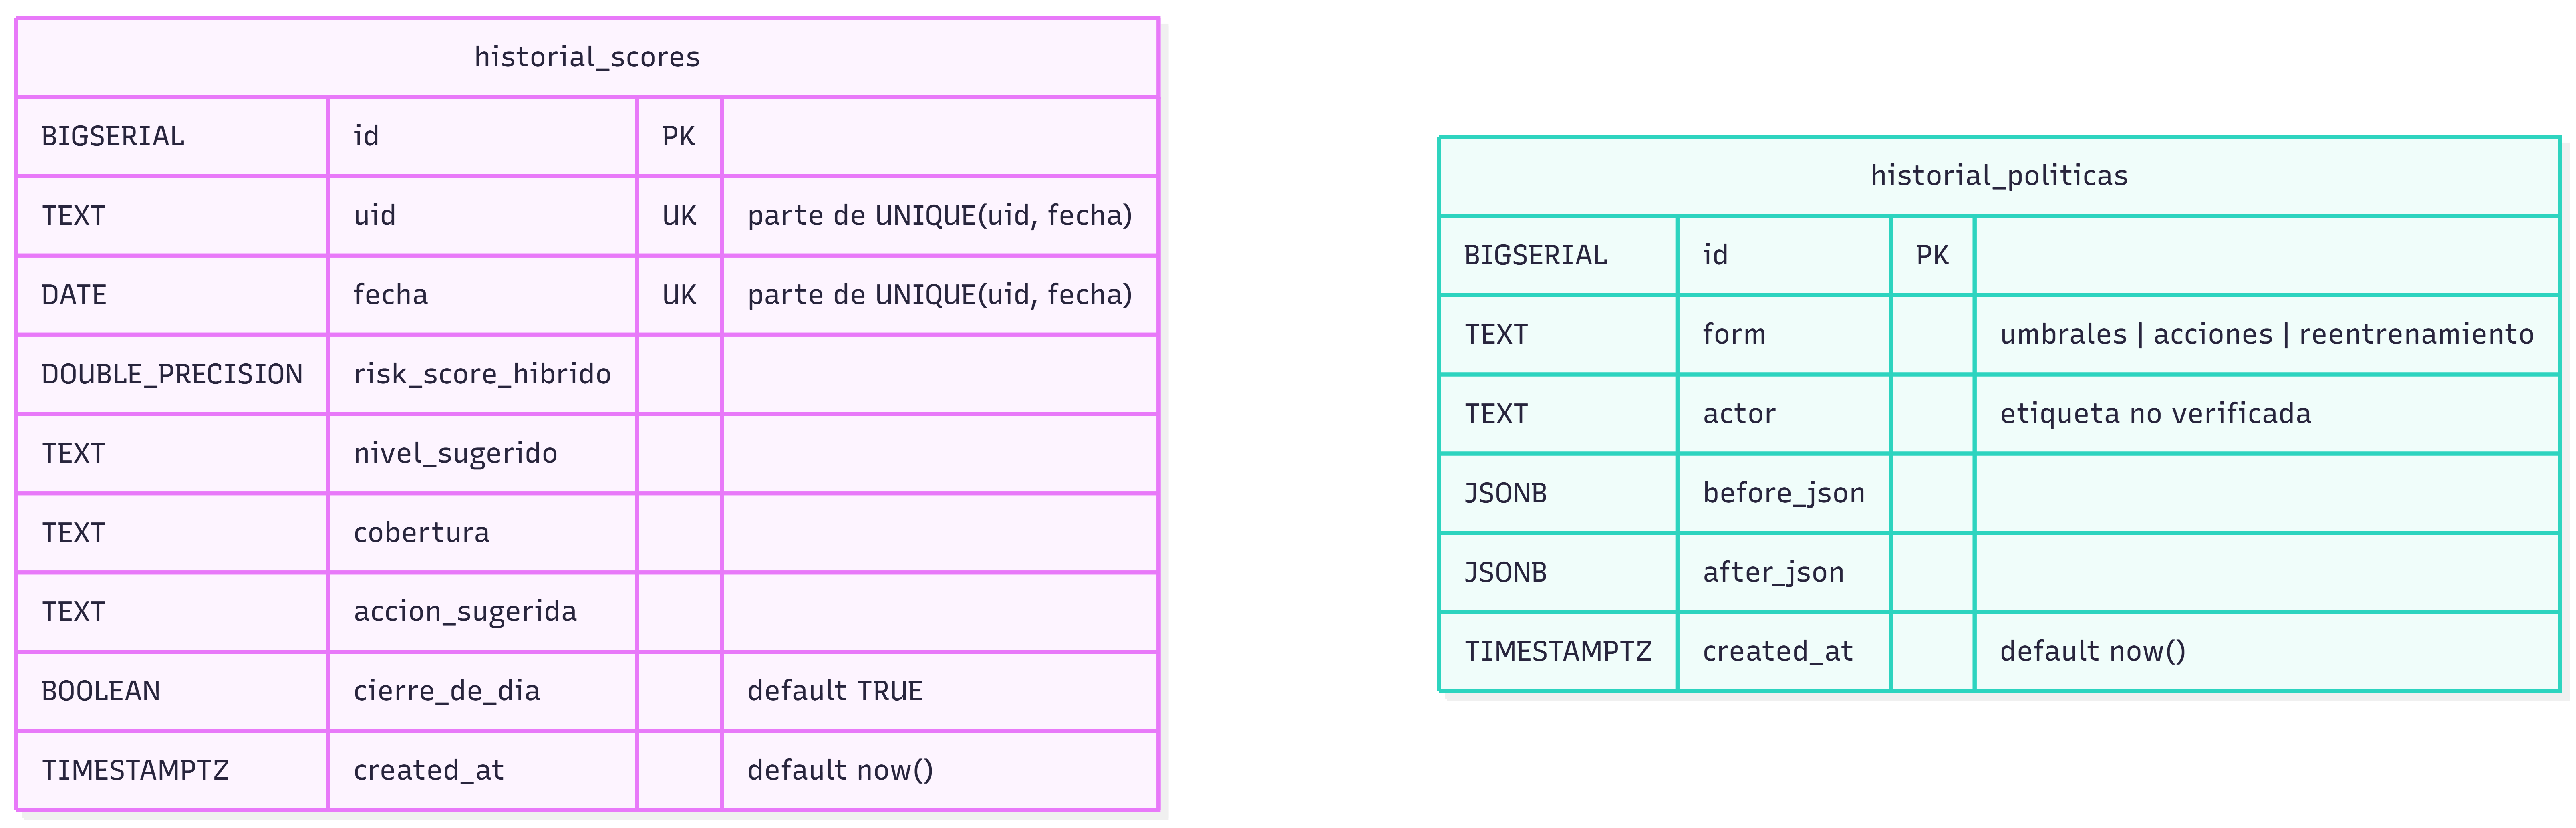
\includegraphics[width=\textwidth]{images/diagramas/supabase.png}
	\caption{Diagrama de Bases de Datos.}
	\label{fig:diagrama-bases-de-datos-supabase}
\end{figure}
\FloatBarrier

\section{Diagrama de Arquitectura}

\begin{figure}[h]
	\centering
	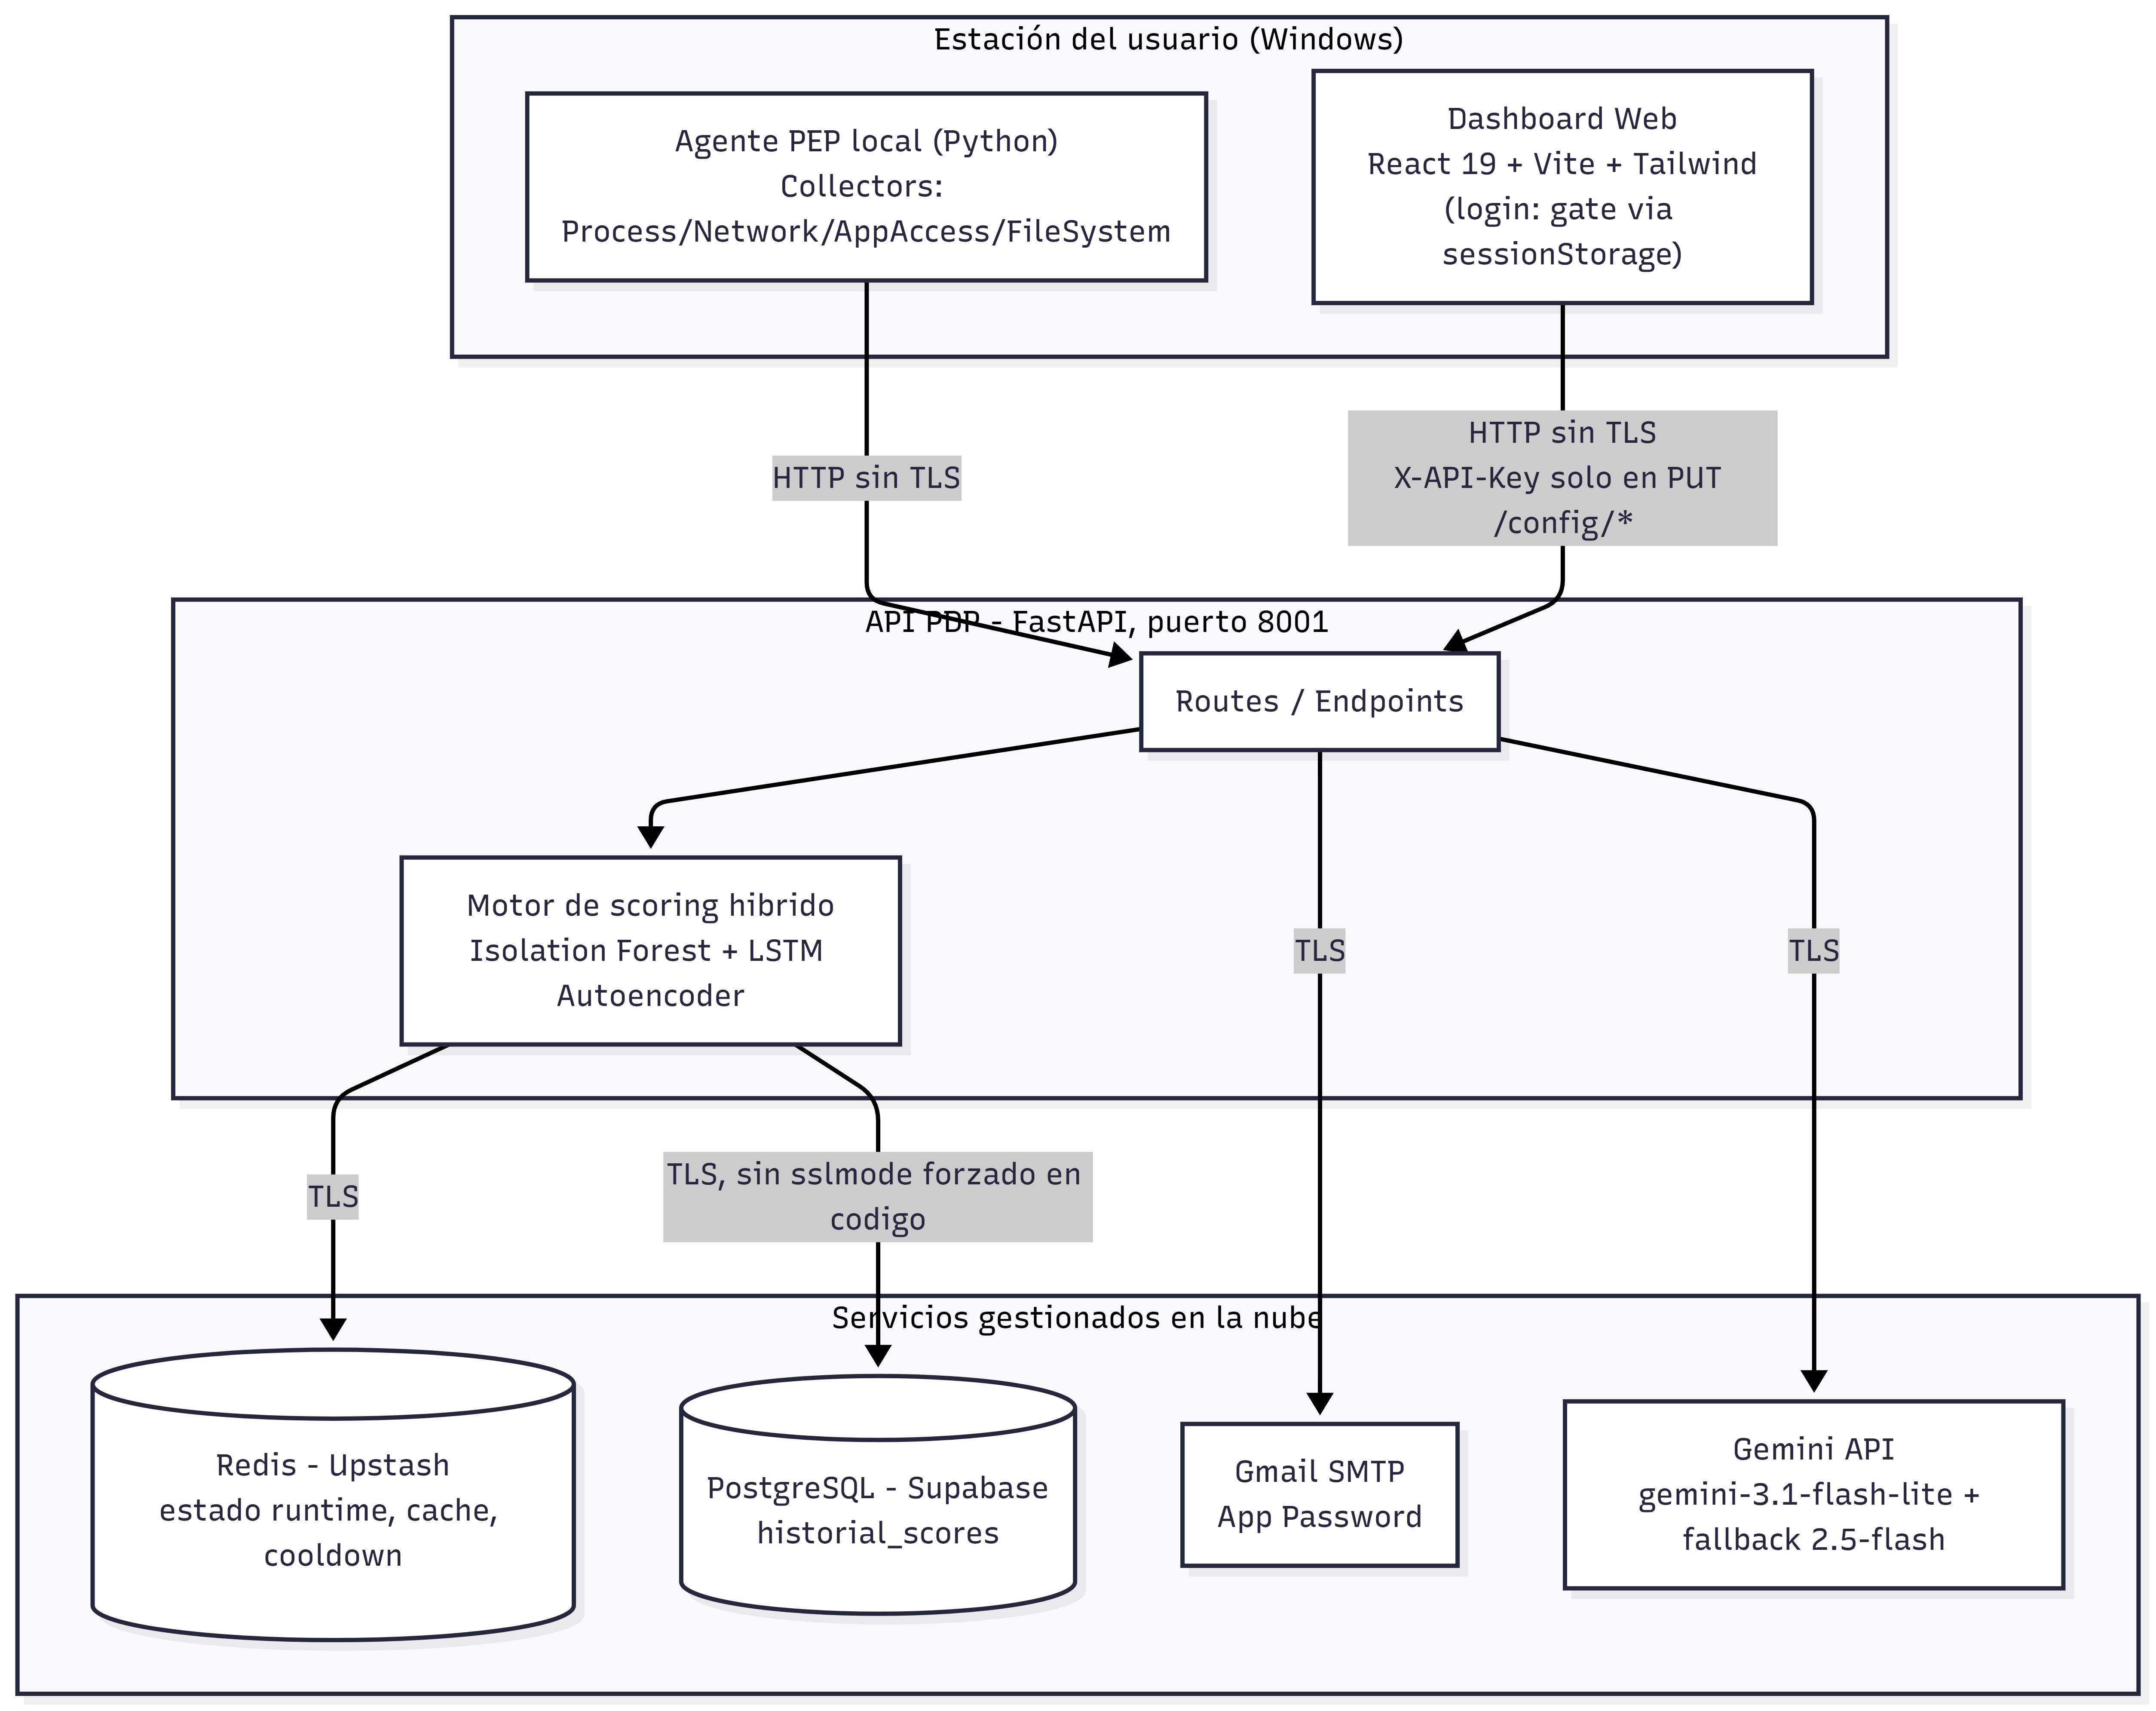
\includegraphics[width=\textwidth]{images/diagramas/diagramaarquitectura.png}
	\caption{Diagrama de Arquitectura del producto.}
	\label{fig:diagrama-arquitectura}
\end{figure}
\FloatBarrier

\clearpage
%%ORIGEN: chapters/chapter03.tex, \chapter{Demo} (líneas 706-fin). Obsoleto, reemplazado por producto.tex
\chapter{Demo}
Este capítulo presenta evidencia funcional del sistema implementado: la documentación interactiva de la API (backend) y las pantallas operativas del \emph{dashboard} (frontend).

\section{Endpoints del Backend (Swagger)}
La API expone su documentación interactiva mediante Swagger/OpenAPI, que permite explorar y probar cada endpoint disponible. A continuación se muestran capturas de dicha documentación.

\begin{figure}[h]
	\centering
	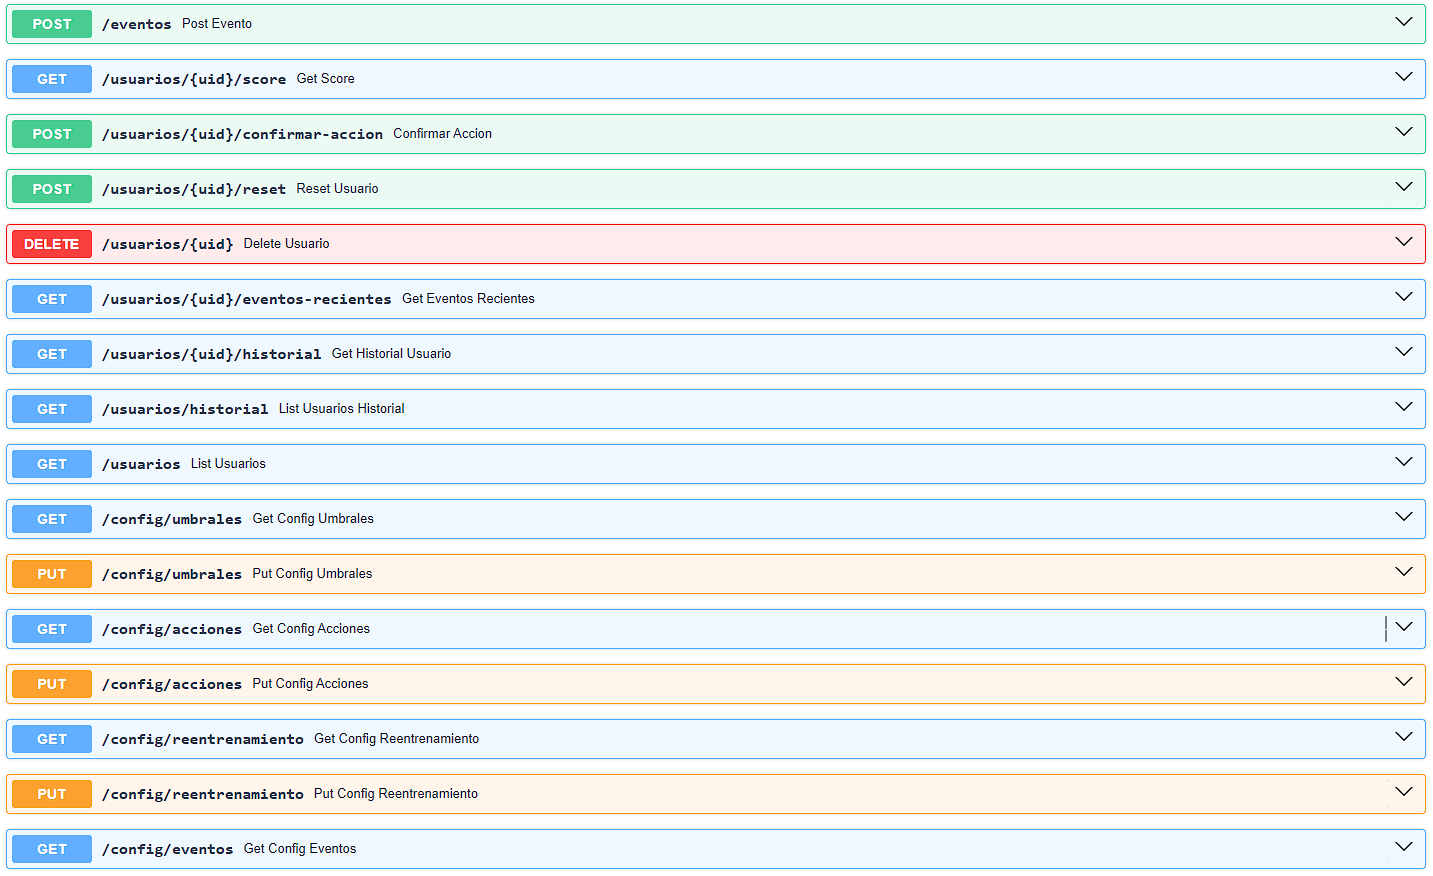
\includegraphics[width=\textwidth]{images/swagger/endpoint1.png}
	\caption{Documentación Swagger de la API — Parte 1.}
	\label{fig:demo-swagger-endpoint1}
\end{figure}
\FloatBarrier

\begin{figure}[h]
	\centering
	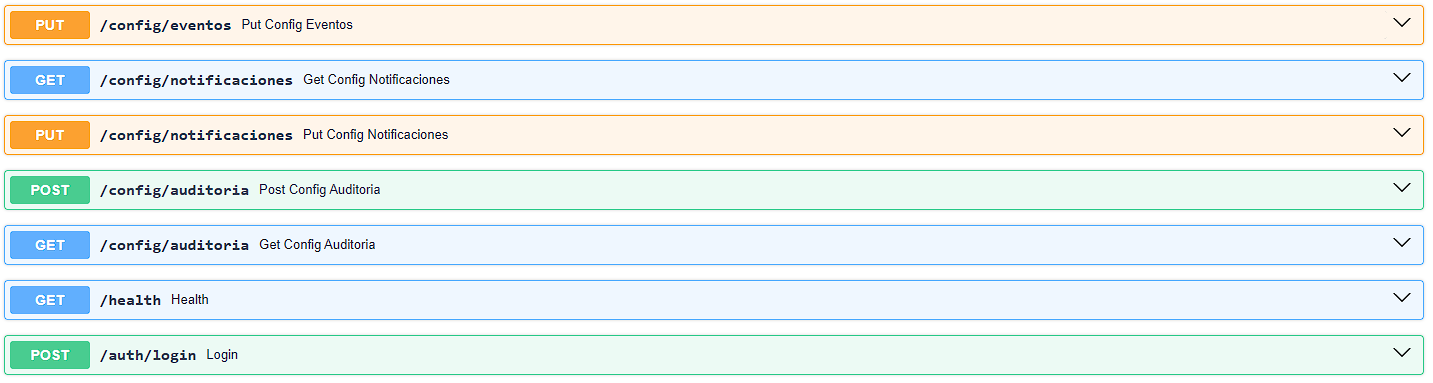
\includegraphics[width=\textwidth]{images/swagger/endpoint2.png}
	\caption{Documentación Swagger de la API — Parte 2.}
	\label{fig:demo-swagger-endpoint2}
\end{figure}
\FloatBarrier

\section{Frontend}
Las capturas de pantalla del frontend, junto con su justificación de diseño y el \emph{wireframe} correspondiente a cada una, se encuentran detalladas en el Capítulo~\ref{sec:decisiones-transversales-mockups} ("Justificación de Diseño y Mockups"). A modo de resumen, se incluyen a continuación las pantallas reales ya implementadas del \emph{dashboard}.

\begin{figure}[h]
	\centering
	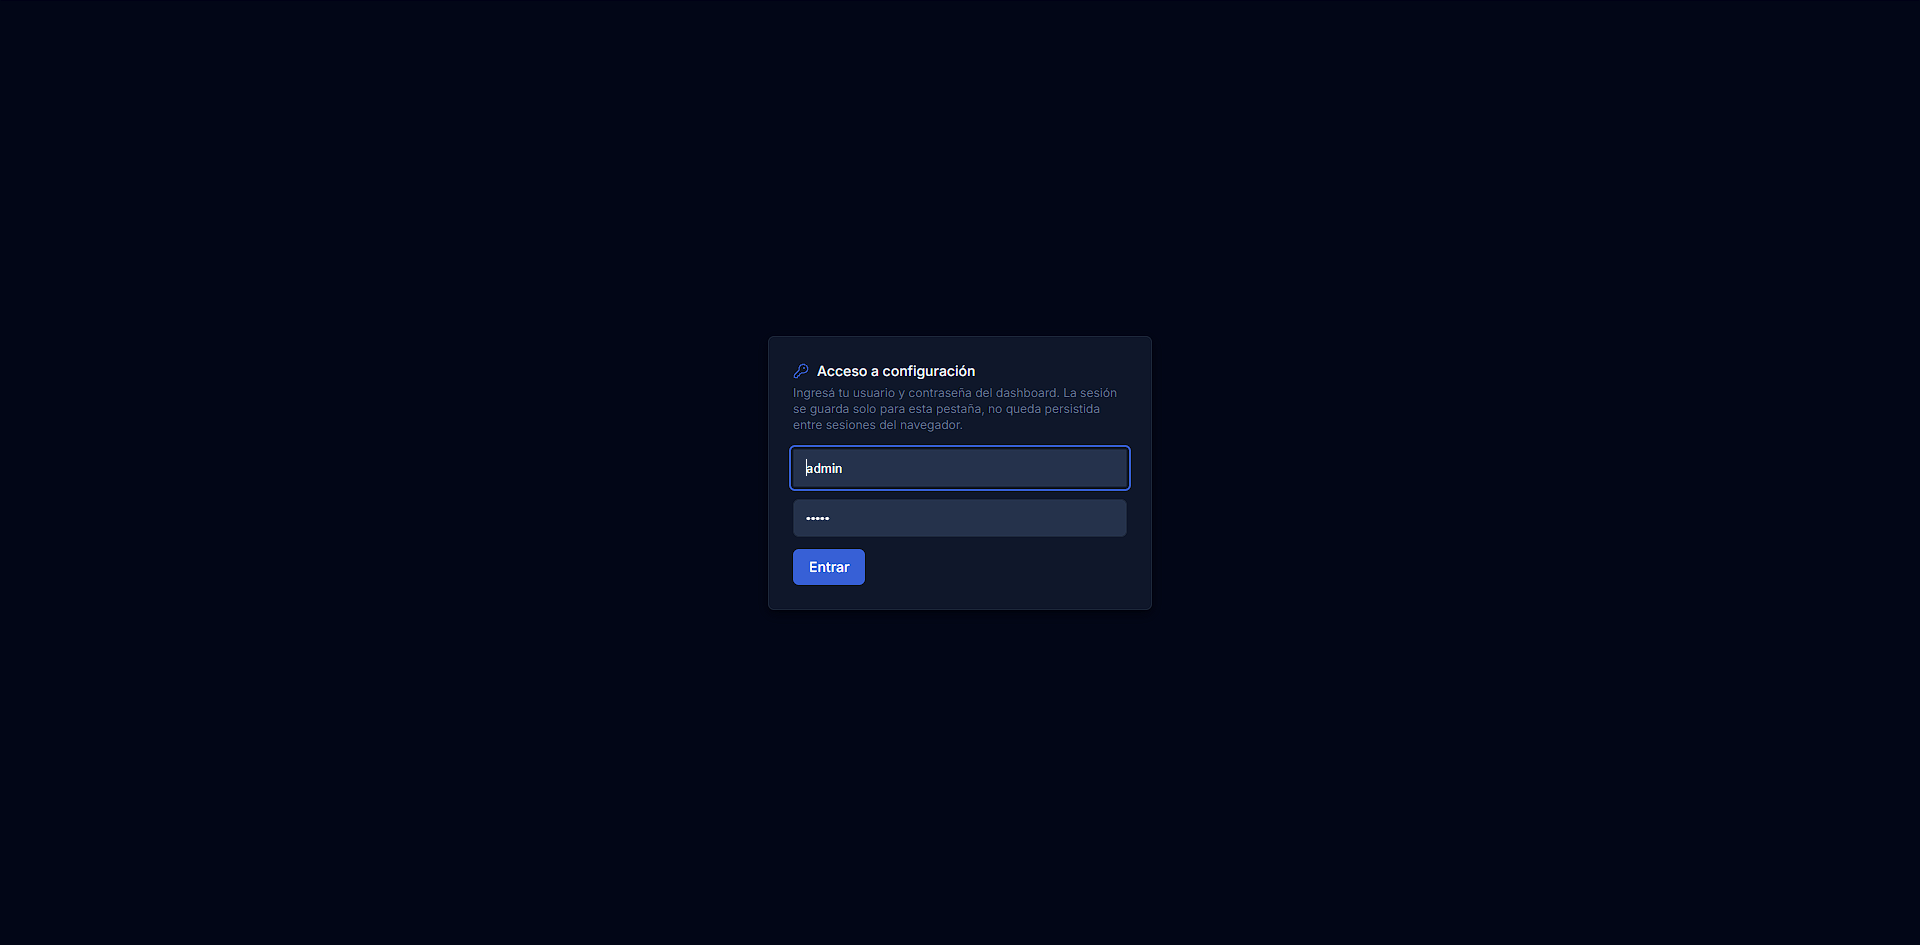
\includegraphics[width=0.8\textwidth]{images/mockups/mockup-login-real.png}
	\caption{Pantalla real: Acceso (Login).}
	\label{fig:demo-mockup-login-real}
\end{figure}
\FloatBarrier

\begin{figure}[h]
	\centering
	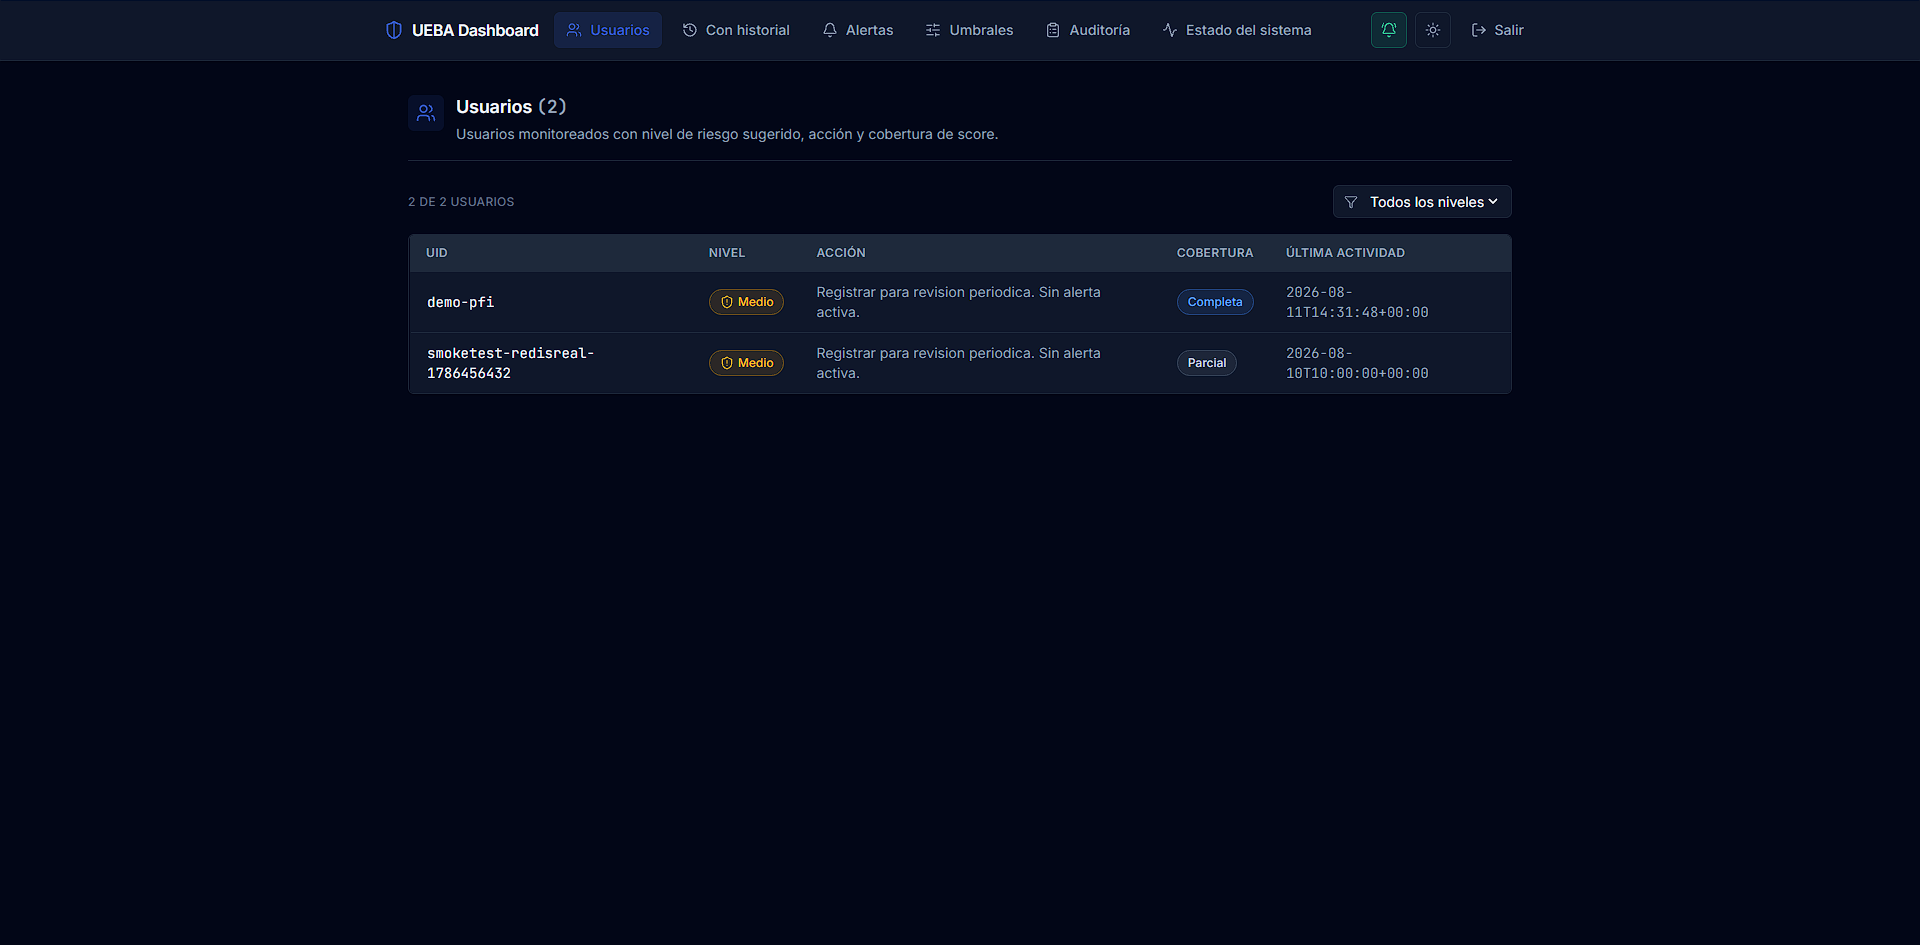
\includegraphics[width=0.8\textwidth]{images/mockups/mockup-usuarios-real.png}
	\caption{Pantalla real: Usuarios.}
	\label{fig:demo-mockup-usuarios-real}
\end{figure}
\FloatBarrier

\begin{figure}[h]
	\centering
	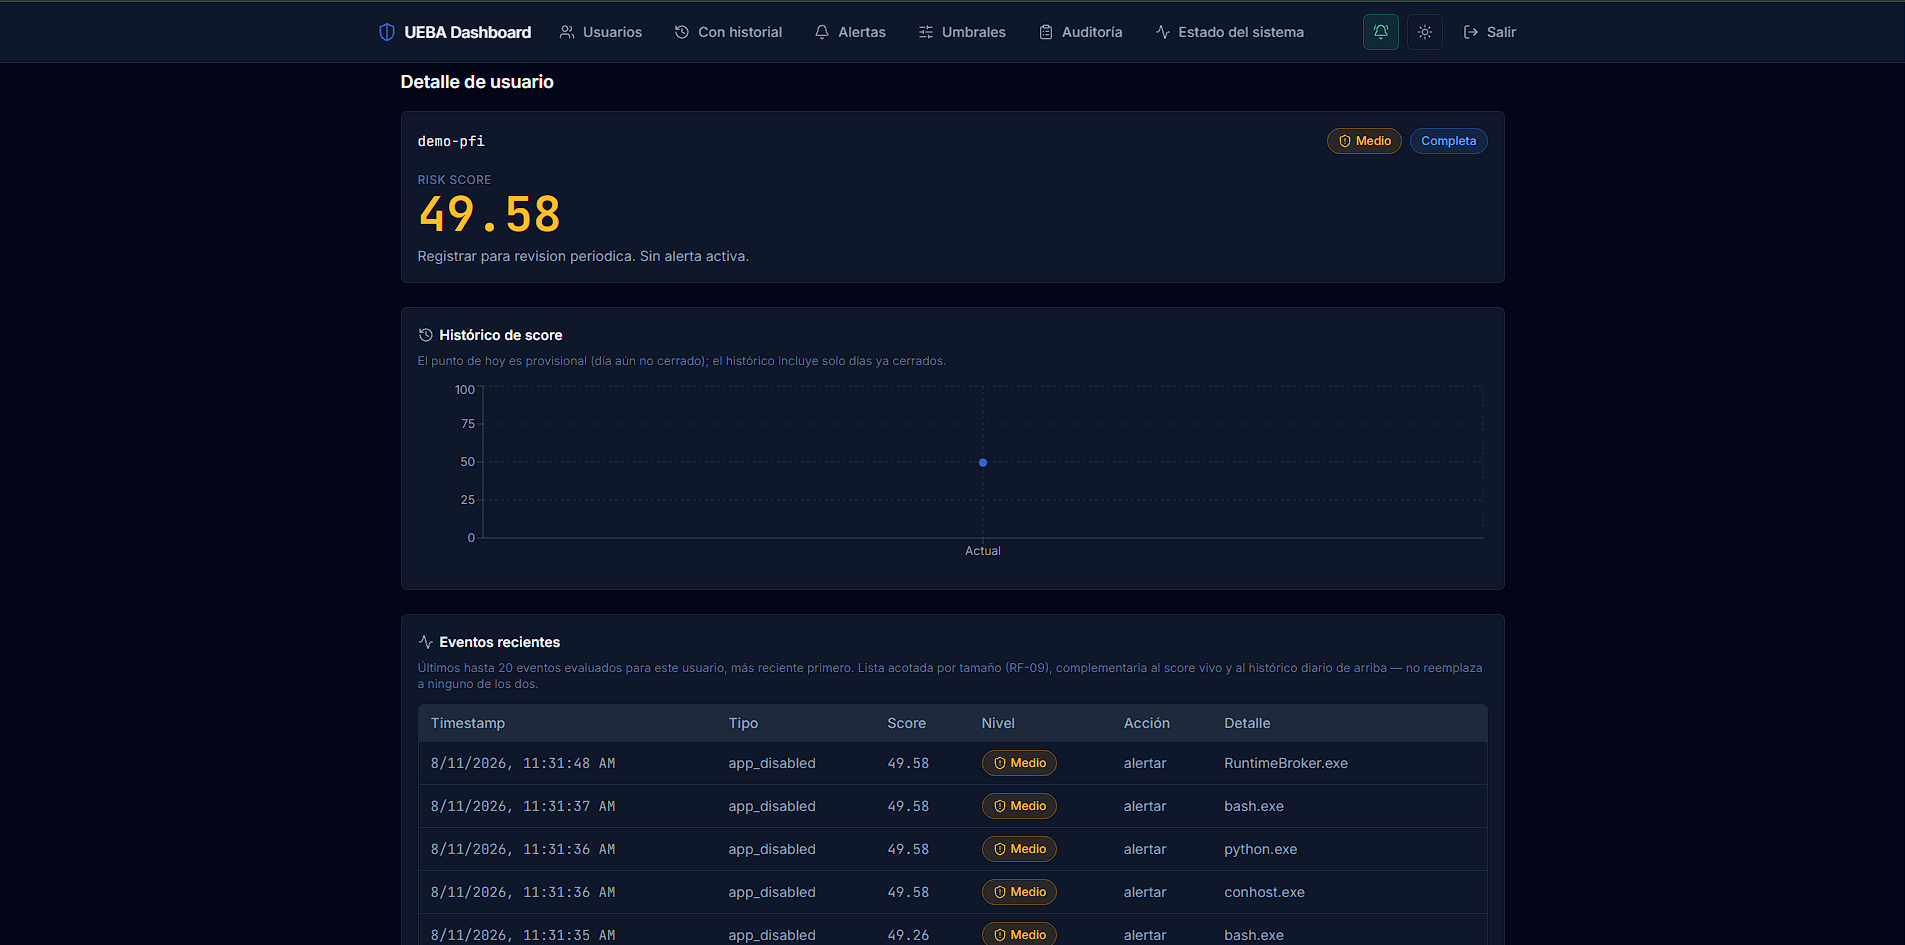
\includegraphics[width=0.8\textwidth]{images/mockups/mockup-detalle-real.png}
	\caption{Pantalla real: Detalle de usuario.}
	\label{fig:demo-mockup-detalle-real}
\end{figure}
\FloatBarrier

\begin{figure}[h]
	\centering
	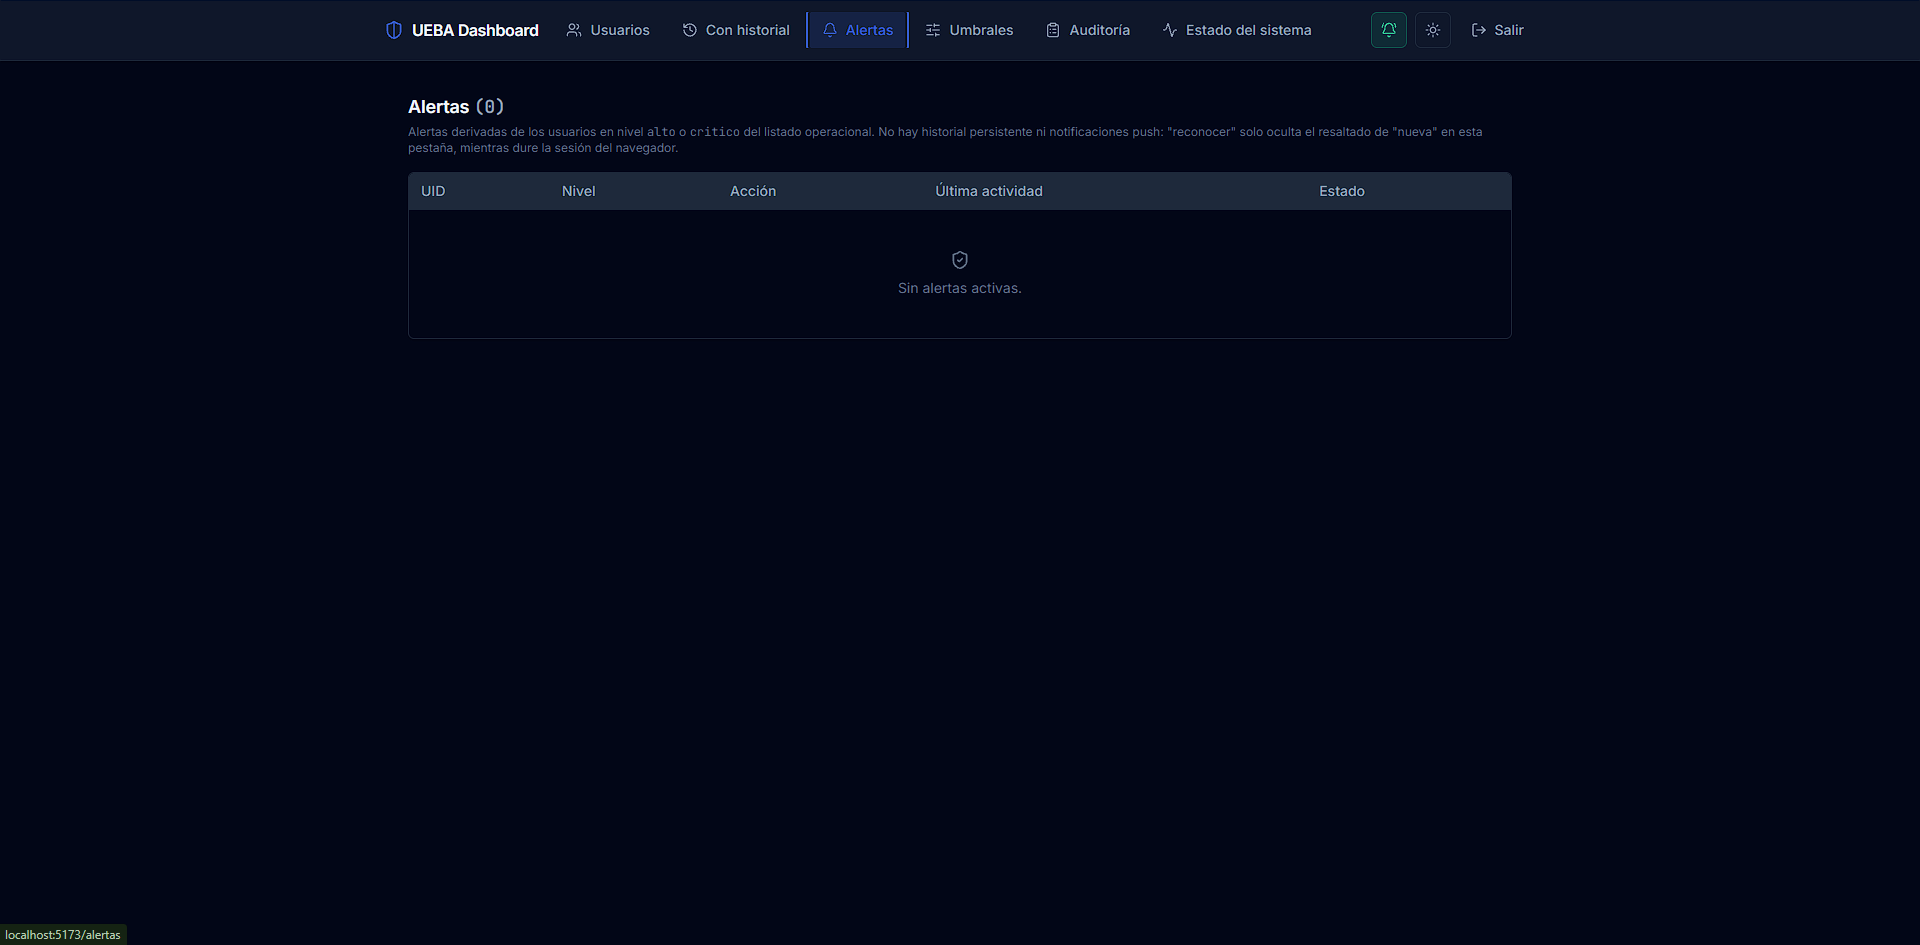
\includegraphics[width=0.8\textwidth]{images/mockups/mockup-alertas-real.png}
	\caption{Pantalla real: Alertas.}
	\label{fig:demo-mockup-alertas-real}
\end{figure}
\FloatBarrier

\begin{figure}[h]
	\centering
	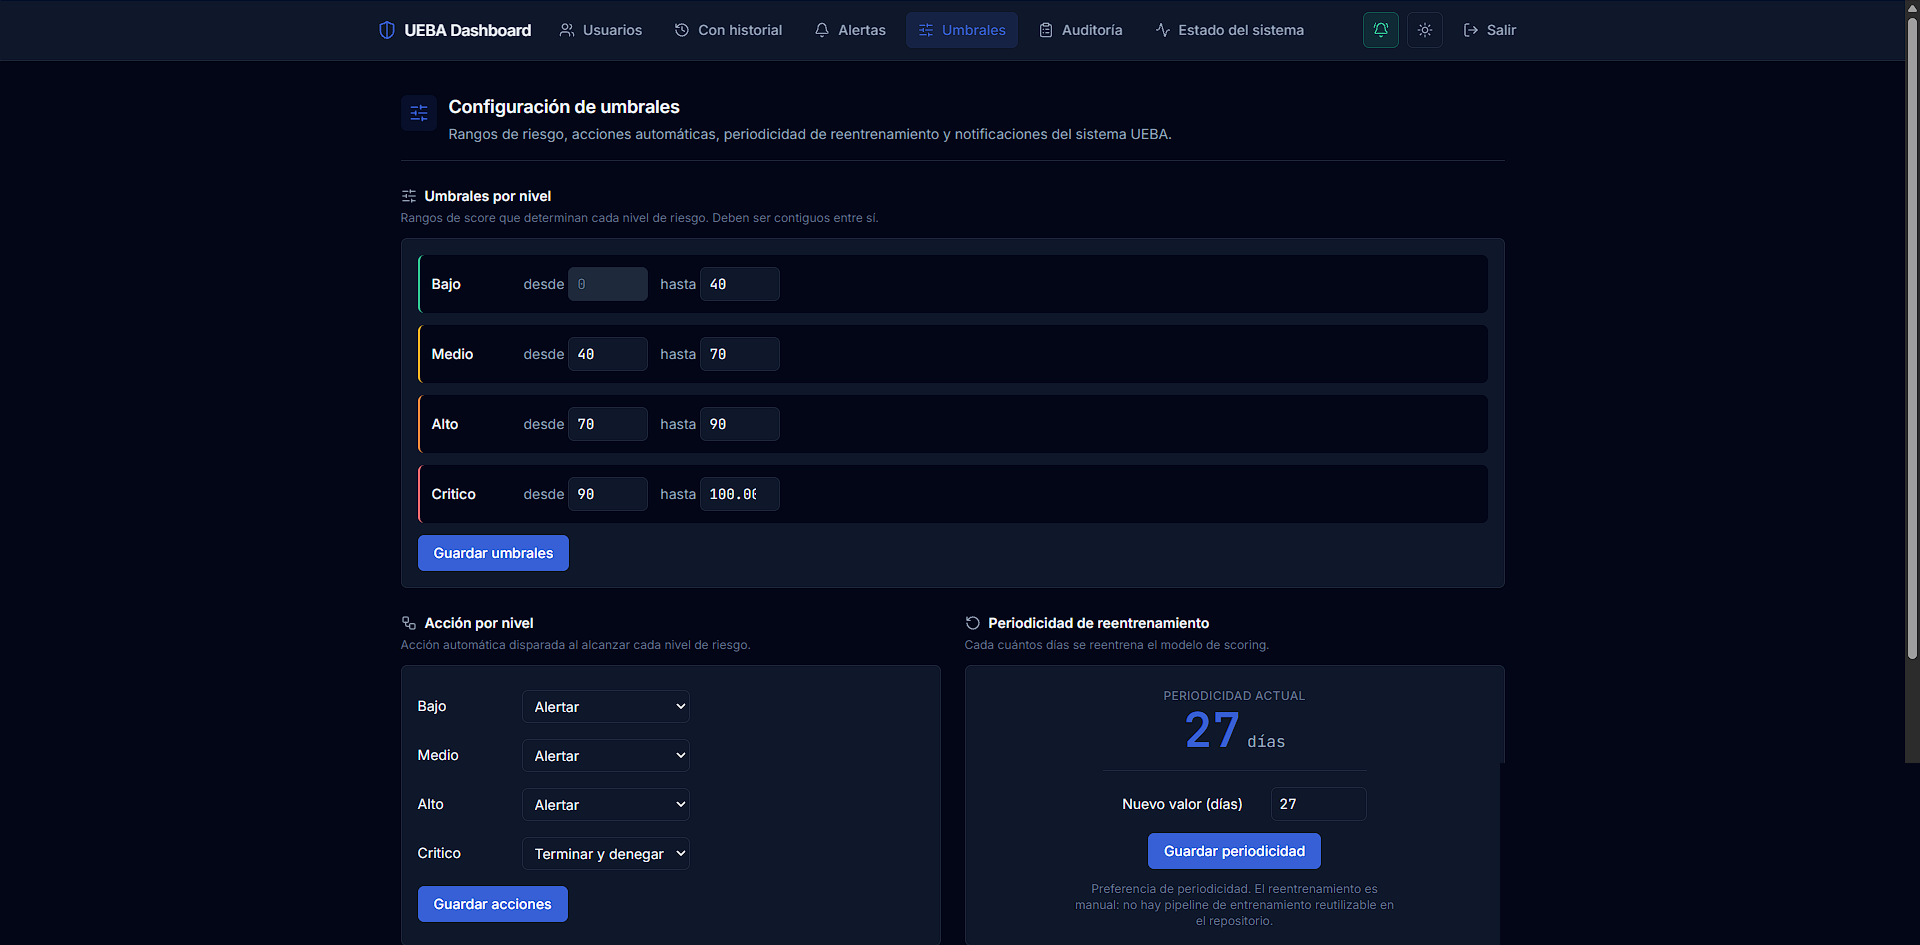
\includegraphics[width=0.8\textwidth]{images/mockups/mockup-umbrales-real-1.png}
	\caption{Pantalla real: Configuración de umbrales (1).}
	\label{fig:demo-mockup-umbrales-real-1}
\end{figure}
\FloatBarrier

\begin{figure}[h]
	\centering
	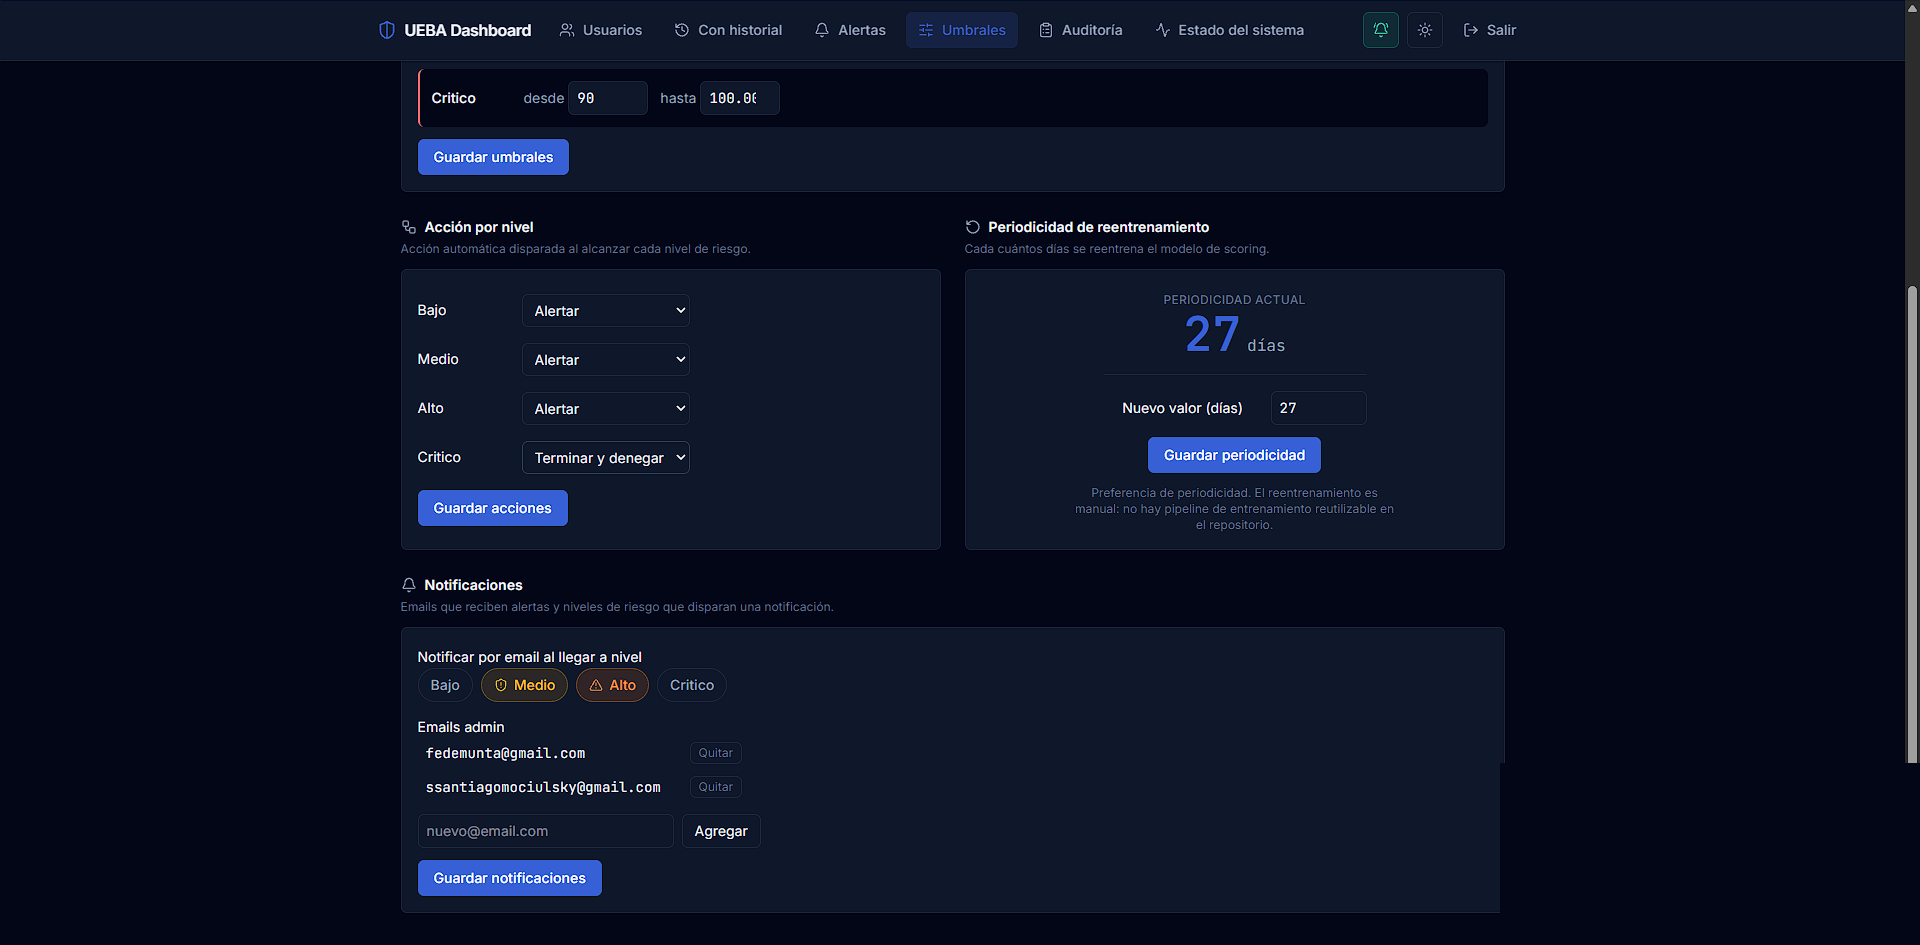
\includegraphics[width=0.8\textwidth]{images/mockups/mockup-umbrales-real-2.png}
	\caption{Pantalla real: Configuración de umbrales (2).}
	\label{fig:demo-mockup-umbrales-real-2}
\end{figure}
\FloatBarrier

\begin{figure}[h]
	\centering
	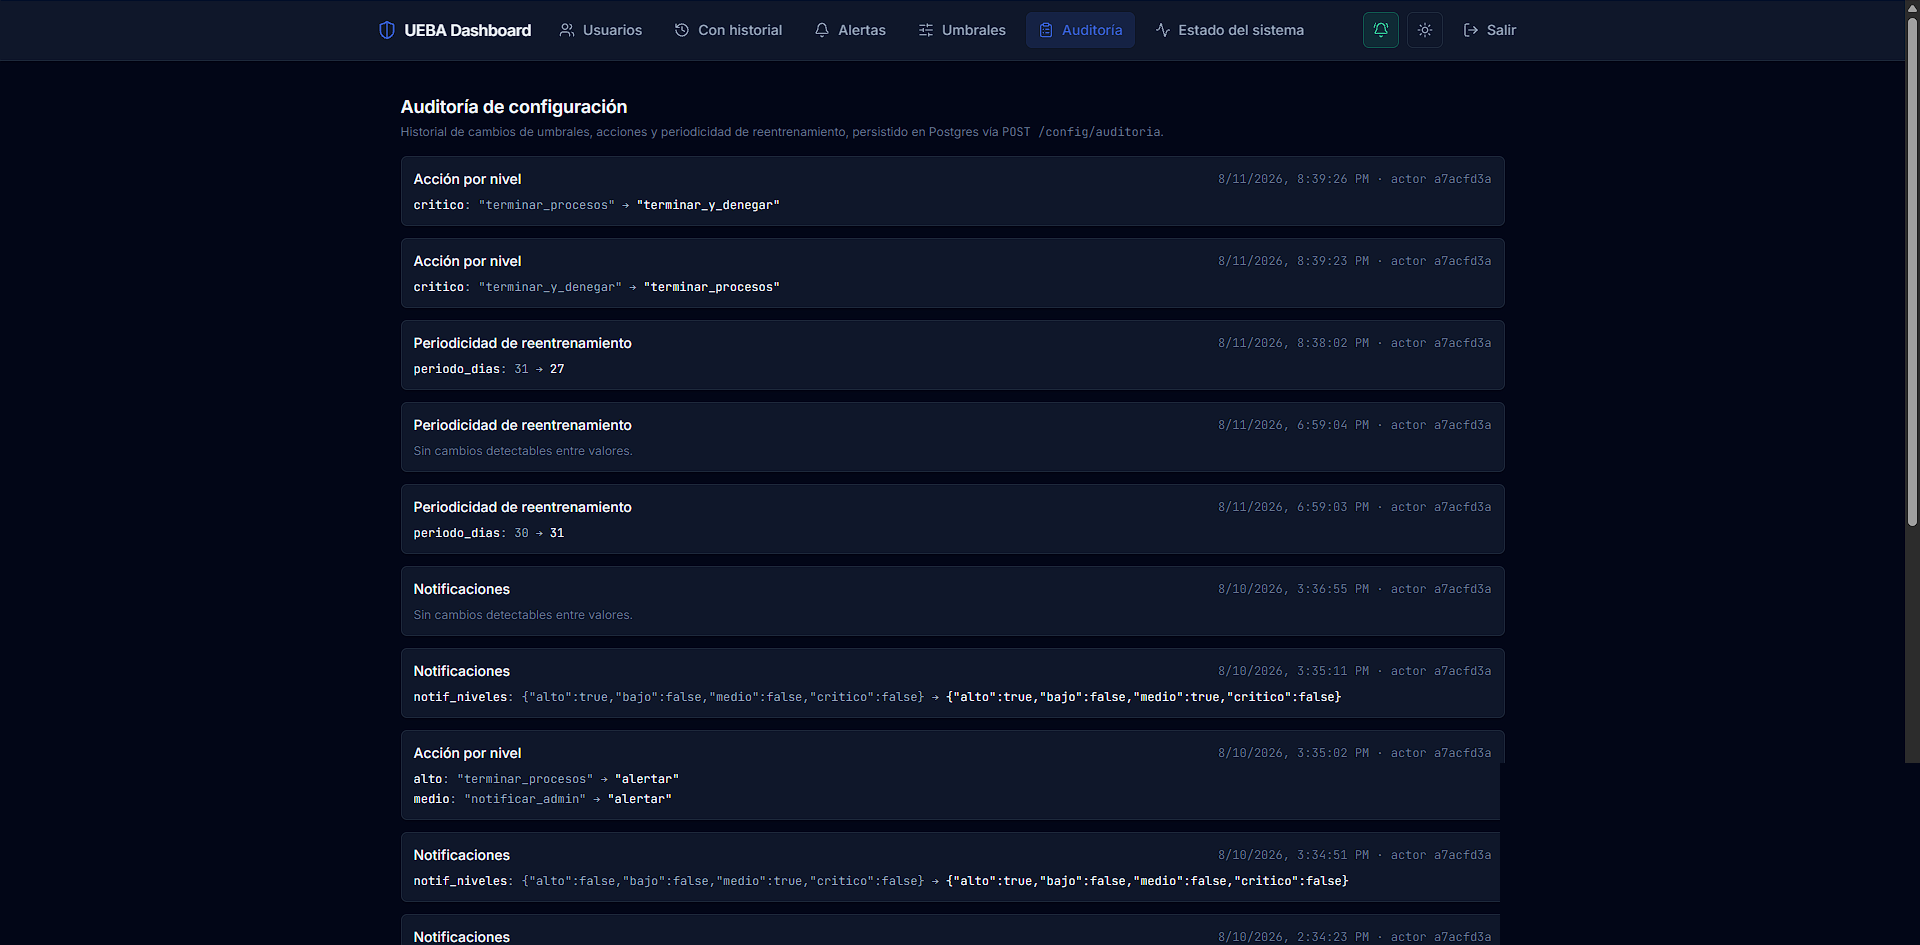
\includegraphics[width=0.8\textwidth]{images/mockups/mockup-auditoria-real.png}
	\caption{Pantalla real: Auditoría.}
	\label{fig:demo-mockup-auditoria-real}
\end{figure}
\FloatBarrier

\begin{figure}[h]
	\centering
	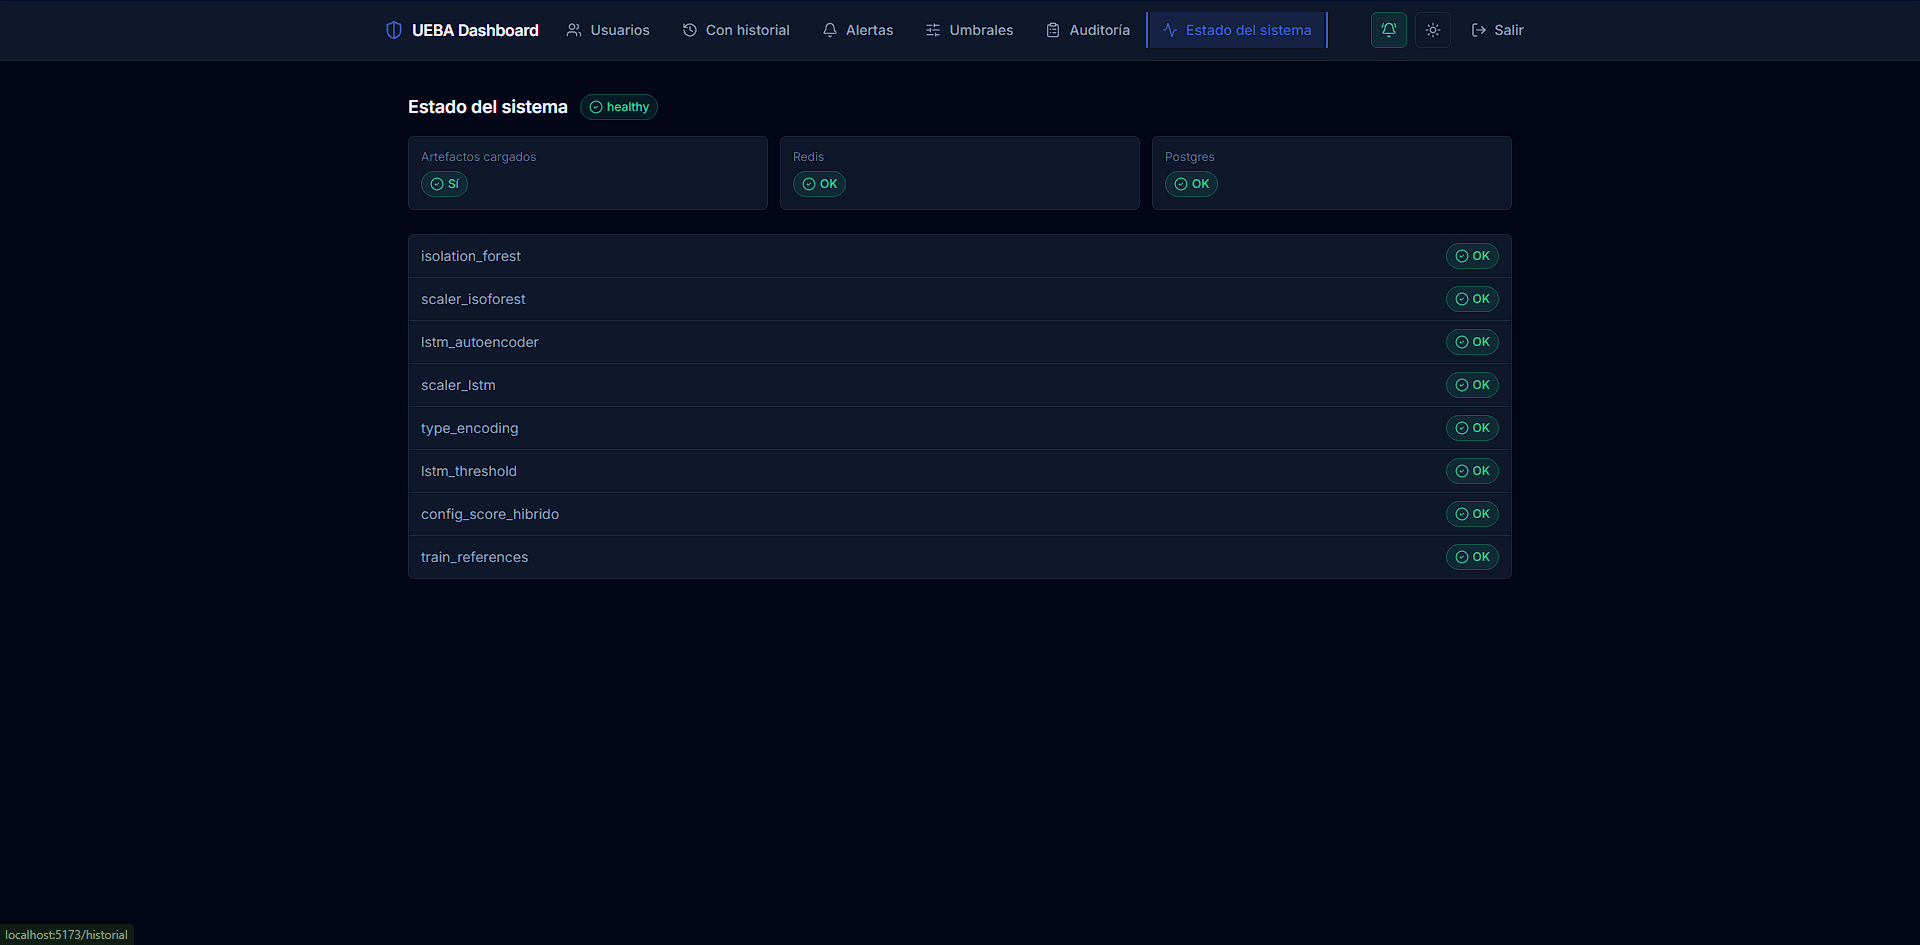
\includegraphics[width=0.8\textwidth]{images/mockups/mockup-estado-real.png}
	\caption{Pantalla real: Estado del sistema.}
	\label{fig:demo-mockup-estado-real}
\end{figure}
\FloatBarrier

\begin{figure}[h]
	\centering
	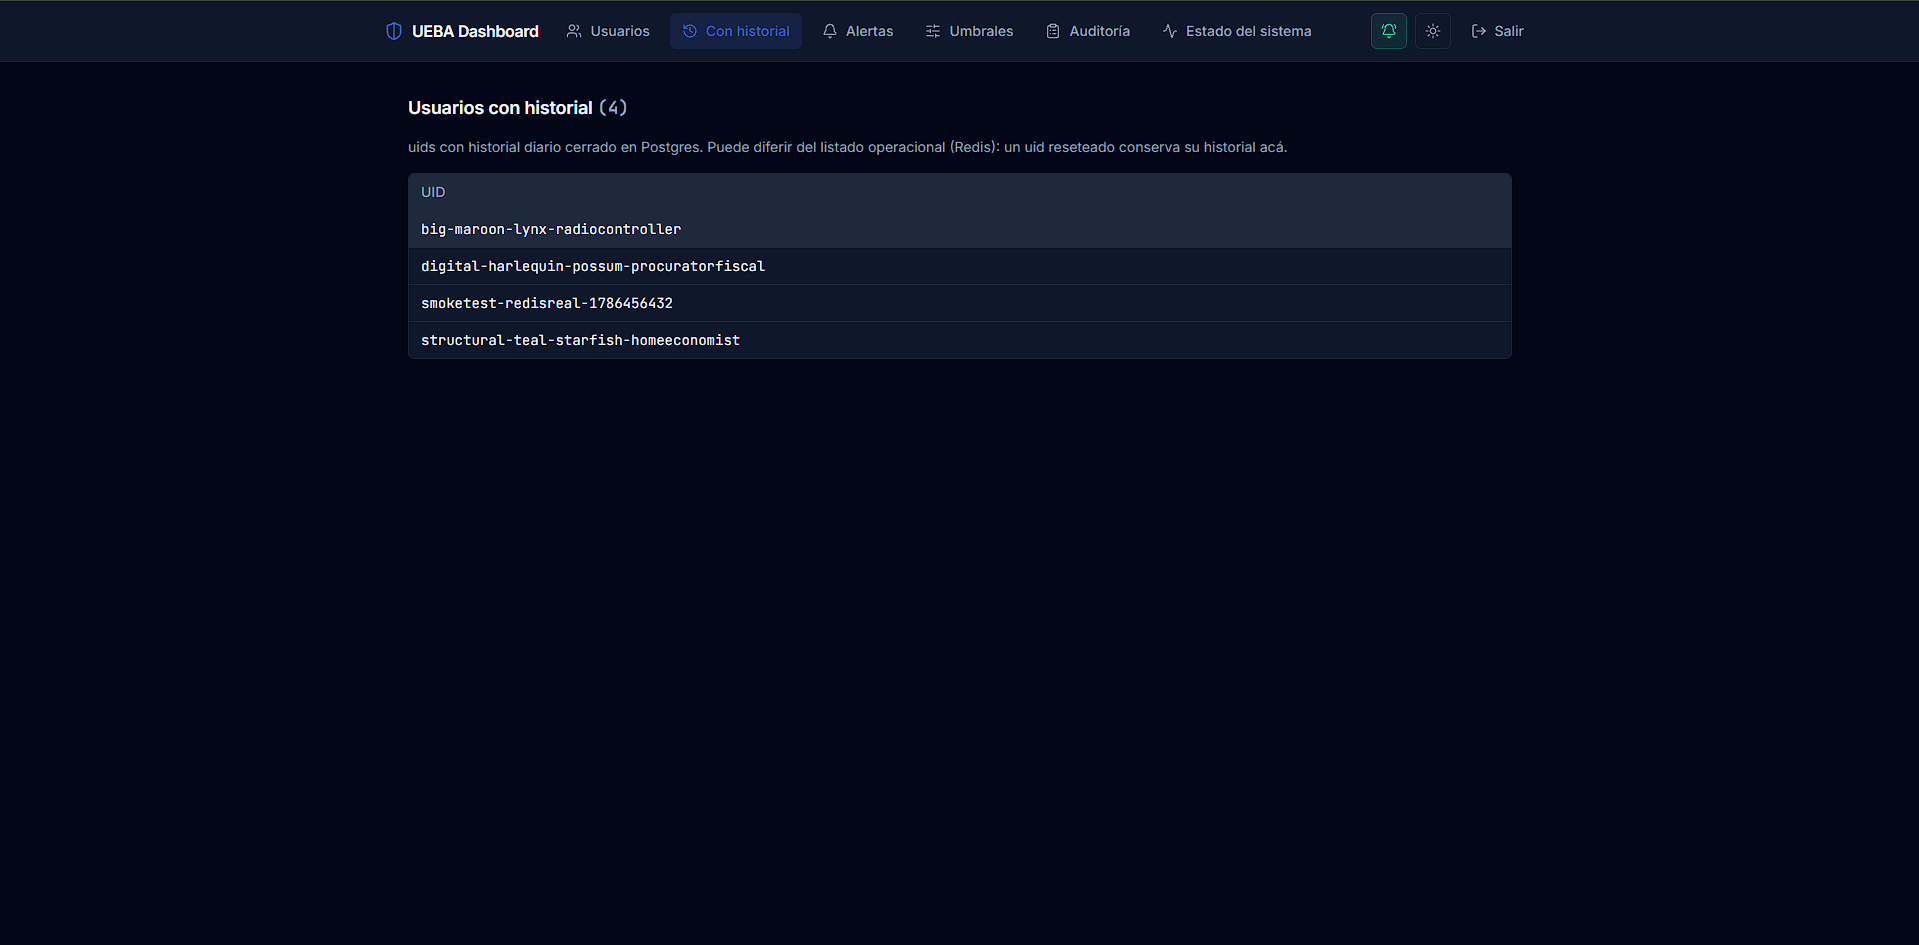
\includegraphics[width=0.8\textwidth]{images/mockups/mockup-historial-real.png}
	\caption{Pantalla real: Con historial.}
	\label{fig:demo-mockup-historial-real}
\end{figure}
\FloatBarrier
%%ORIGEN: chapters/chapter02.tex, \subsection{El Dataset CLUE-LDS} (2.2.6, líneas 230-235). Obsoleto, reemplazado por datos.tex
\subsection{El Dataset CLUE-LDS}
Para el desarrollo y la validación del presente sistema se utiliza el dataset CLUE-LDS (\emph{Cloud-based User Entity Behavior Analytics Log Data Set}), una colección de logs de producción diseñada específicamente para su aplicación en UEBA \parencite{Landauer2022Dataset}. A diferencia de la mayoría de los datasets disponibles públicamente en este dominio, los registros de CLUE-LDS provienen del uso cotidiano real de clientes de Huemer Group, un proveedor mediano de servicios de TI con sede en Viena, Austria. La única transformación aplicada a los datos originales fue la anonimización de identificadores (como nombres de usuario y direcciones IP) mediante su reemplazo por valores ficticios, preservando en todo momento la coherencia y la continuidad de los patrones de comportamiento de cada entidad. 

En términos de magnitud, el dataset contiene aproximadamente 50 millones de eventos generados por más de 5.000 usuarios únicos anonimizados, distribuidos a lo largo de más de cinco años de actividad continua, desde el 7 de julio de 2017 hasta el 29 de septiembre de 2022. Esta ventana temporal resulta especialmente valiosa para el análisis de comportamiento, ya que permite identificar tendencias estacionales, cambios de rol y evoluciones graduales en los patrones de uso que difícilmente podrían observarse en datasets de menor duración. 

Desde el punto de vista estructural, los datos se encuentran en formato JSON, donde cada línea corresponde a un objeto JSON independiente que representa un evento del sistema. Cada registro incluye un identificador numérico secuencial (\texttt{id}), una marca temporal en formato ISO UTC (\texttt{time}), un identificador anonimizado de la entidad que generó el evento (\texttt{uid}) y su tipo asociado (\texttt{uidType}), lo que permite diferenciar entre usuarios autenticados y direcciones IP de acceso no autenticado. El campo \texttt{type} almacena la acción ejecutada, como \texttt{file\_accessed} o \texttt{login\_successful}, mientras que \texttt{params} contiene un conjunto de parámetros cuya estructura varía según el tipo de evento e incluye información como rutas de archivos, nombres de carpetas o grupos involucrados. Además, algunos registros incorporan campos opcionales que aportan mayor contexto al evento. Entre ellos, \texttt{isLocalIP} indica si la conexión se originó dentro o fuera de la red corporativa; \texttt{role} identifica el rol laboral del usuario, con categorías como administración, consultoría, ventas, gestión, técnico o externo; y \texttt{location} proporciona información de geolocalización obtenida a partir de la IP de origen, incluyendo país, región, ciudad, coordenadas geográficas y huso horario.
